\documentclass[11pt,letterpaper]{article}

% --- Typography & Page Layout ---
\usepackage[margin=1in]{geometry}
\usepackage{setspace}
\onehalfspacing
\usepackage[T1]{fontenc}
\usepackage[utf8]{inputenc}
\usepackage{microtype}
\usepackage{lmodern}

% --- Math Packages ---
\usepackage{amsmath,amssymb,amsfonts,bm}
\usepackage{mathtools}

% --- Tables & Figures ---
\usepackage{booktabs}
\usepackage{tabularx}
\usepackage{array}
\usepackage{makecell}
\usepackage{graphicx}
\usepackage[font=small,labelfont=bf,tableposition=top]{caption}
\usepackage{subcaption}

% --- Colors & Hyperlinks ---
\usepackage[dvipsnames]{xcolor}
\usepackage[colorlinks=true,linkcolor=MidnightBlue,citecolor=MidnightBlue,urlcolor=MidnightBlue]{hyperref}

% --- Citations (Nature style superscript numbers) ---
\usepackage[super,sort&compress]{natbib}

% --- Custom Math Notation ---
\newcommand{\JSD}{\operatorname{JSD}}
\newcommand{\dself}{d_{\mathrm{self}}}
\newcommand{\dref}{d_{\mathrm{ref}}}
\newcommand{\Turnover}{\mathrm{Turnover}}
\newcommand{\Jaccard}{\mathrm{Jaccard}}

\title{\textbf{Examining the Relational Content and Personal Determinants of Social Signatures Across Multiple Time Scales}}

\author{
  Omar Lizardo$^{1,*}$ \and David Hachen$^{2}$
}

\date{}

\begin{document}

\maketitle

\noindent
$^{1}$Department of Sociology, University of California, Los Angeles, Los Angeles, CA 90095, USA.\\
$^{2}$Department of Sociology, University of Notre Dame, Notre Dame, IN 46556, USA.\\
$^{*}$Corresponding author: \texttt{olizardo@soc.ucla.edu}

\vspace{1.5em}

\begin{abstract}
\noindent
How do individuals allocate cognitive, temporal, and emotional bandwidth across personal networks? Using passive smartphone logs and eight longitudinal survey waves from the NetHealth study ($N = 491$ egos, 498,237 calls), we examine the structure, temporal stability, and psychological foundations of social signatures---the ranked allocation of communication across contacts. Signature persistence endures across multiple calendar and rolling timescales ($p < 0.0001$), with power-law decay models outperforming exponential specifications and parameter estimates stabilizing within six to eight months. Linking communication ranks to ego-network surveys ($N = 13,174$ dyads) reveals that interaction drop-off tracks sharp relational transitions from kinship-dominated instrumental and emotional support at primary ranks to peer companionship in outer bands. Furthermore, signature stability persists despite 80.1\% semester-to-semester alter turnover, confirming that individuals slot new entrants into pre-existing relational positions. Finally, elevated Negative Emotionality strongly predicts hyper-concentrated signatures, with Extraversion acting as a non-linear buffer against relational withdrawal.
\end{abstract}

\vspace{1em}
\noindent\textbf{Keywords:} Social Signatures; Egocentric Networks; NetHealth; Tie Strength; Slot-Filling Hypothesis; Personality Traits; Mobile Sensing.

\newpage

% --- Introduction (No Section Heading in Nature Human Behaviour) ---

A central puzzle in the scientific study of human sociality is the tension between relational fluidity and structural constraint.\cite{mcpherson2001birds-2dc,rivera2010dynamics-e3e} Across the life course, individuals move through dynamic, evolving social worlds: entering new institutions, forming partnerships, making new friends, and allowing older ties to lapse.\cite{suitor1997its-18f} Yet despite the continual turnover of interaction partners, personal communication behavior is not randomly distributed across contacts, nor does it restructure arbitrarily when network composition changes. Instead, relational investment is bounded by deep-seated cognitive and temporal constraints on sociality.\cite{dunbar1992neocortex,dunbar1998social,miritello2013time} While individuals can recognize hundreds of faces and maintain casual awareness of extensive social circles, active personal networks are structured into concentric, hierarchical layers: an intimate support clique of 1 to 2 confidants, a sympathy group of approximately 5 close ties, an affinity group of 12 to 15 regular contacts, and expanding outer bands of declining emotional intensity and contact frequency.\cite{dunbar2018anatomy,roberts2009exploring,sutcliffe2012relationships} Because time is a non-renewable, zero-sum budget, individuals cannot allocate attention uniformly across their contacts; investing heavily in one relationship inevitably constrains the bandwidth available for others.\cite{miritello2013time}

In a seminal contribution, Saram{\"a}ki and colleagues\cite{saramaeki2014persistence} characterized this relational hierarchy using the concept of \textit{social signatures}, namely, the probability distribution of communication effort that an individual (ego) directs toward their contacts (alters), ordered from most to least frequently contacted within a given observation window. Tracking young adults transitioning from high school to university using mobile call records, Saram{\"a}ki and colleagues\cite{saramaeki2014persistence} uncovered two fundamental regularities: first, social signatures exhibit marked \textit{interindividual variation}, ranging from steep, hyper-concentrated profiles focused on a single alter to broad, egalitarian allocations; and second, an individual's social signature displays remarkable \textit{intraindividual persistence} over time. Crucially, this persistence held even when personal networks underwent substantial turnover, prompting Saram{\"a}ki and colleagues\cite{saramaeki2014persistence} to hypothesize a ``slot-filling'' dynamic in which individuals maintain stable cognitive slots and replenish them with new alters as old relationships fade.

Over the past decade, a rich multidisciplinary literature has expanded upon this framework. Researchers have confirmed signature persistence across diverse communication channels, including text messaging,\cite{heydari2018multichannel} online collaborative platforms,\cite{li2018social,koltsova2021social} and in-person sensor networks.\cite{li2022evidence,adel2026preferentiality} Physicists and network scientists have developed continuous resource allocation models\cite{tamarit2022beyond} and generative micro-foundations rooted in the competition between cumulative advantage and random exploration,\cite{iniguez2023universal} while methodological refinements have confirmed that signature persistence reflects genuine tie strength heterogeneity rather than network size stability.\cite{heydari2024disentangling,heydari2024dynamic} Recent inquiries have even shown that signature distinctiveness is so pronounced that communication profiles function as behavioral biometric fingerprints.\cite{jia2025multidimensional}

Despite these advances, the literature has encountered a persistent empirical impasse defined by several open questions. Most critically, because previous investigations have relied almost exclusively on commercial telecommunications metadata or passive digital traces,\cite{saramaeki2014persistence,heydari2018multichannel,iniguez2023universal} researchers have encountered a severe \textit{content black box}: commercial logs record the timing and frequency of calls, but contain zero information regarding dimensions of social support, emotional content, or the relational foundations of the underlying relationships.\cite{burt1985relation,wellman1990different-b11} Does the steep drop-off between Rank 1 and lower-ranked alters correspond to qualitative distinctions in social support, such as emotional comfort, instrumental advice, companionship, or financial aid? Furthermore, the behavioral mechanism governing signature stability remains empirically unverified: does signature persistence truly reflect active ``slot-filling,'' or does it merely mirror the retention of core ties? Finally, what psychological dispositions and personality traits account for the deep interindividual variation observed in signature steepness? Extant models hypothesize that internal cognitive traits drive alter-preferentiality \cite{dunbar2018anatomy,iniguez2023universal} but commercial call records lack psychometric data.

This study addresses these questions by analyzing data from \textit{NetHealth}---a comprehensive longitudinal cohort study tracking an incoming class of undergraduate students at the University of Notre Dame across two full academic years.\cite{liu2018network,purta2016experiences,faust2017exploring,liu2021heterogeneous} By pairing continuous smartphone call records ($N = 491$ egos; 498,237 communication events) with an academic calendar, eight waves of longitudinal ego-network surveys ($35,913$ alter nominations), complete alter-alter structural edge lists ($174,748$ ties), and longitudinal psychometric batteries (Big Five personality traits), we conduct an empirical investigation of the structure, correlates, and determinants of social signatures. Specifically, we evaluate signature persistence across multiple calendar and rolling timescales, test parametric power-law versus exponential scaling, establish the observation duration required for parameter convergence, ground communication ranks in multidimensional social support dimensions, test the slot-filling dynamic under top-alter turnover, and estimate the psychological and structural drivers of signature morphology.

\section*{Results}

\subsection*{Signature morphology and persistence across timescales}

To establish whether personal communication allocations exhibit consistent morphological properties, we evaluated empirical social signatures across eight distinct temporal window schemes, spanning calendar resolutions (academic years, semesters, quarters, months) and rolling weekly intervals (3-week rolling, 2-week discrete, 1-week discrete; see Extended Data Table~\ref{tab:cohort_summary} for cohort inclusion details). 

Figure~\ref{fig:mean_signatures} displays empirical social signatures averaged across participants for ranks 1 through 15 across temporal window definitions. Across all timescales, communication effort exhibits pronounced, heavy-tailed skewness. The single top-ranked alter ($r = 1$) commands 35\% to 45\% of an ego's total communication bandwidth, while the second-ranked alter ($r = 2$) captures between 18\% and 22\%. Together, the top three alters account for over 70\% of total outgoing interaction volume. Beyond rank 5, communication drops below 4\% per alter, forming a prolonged, thin tail of occasional contacts.

\begin{figure}[htbp]
\centering
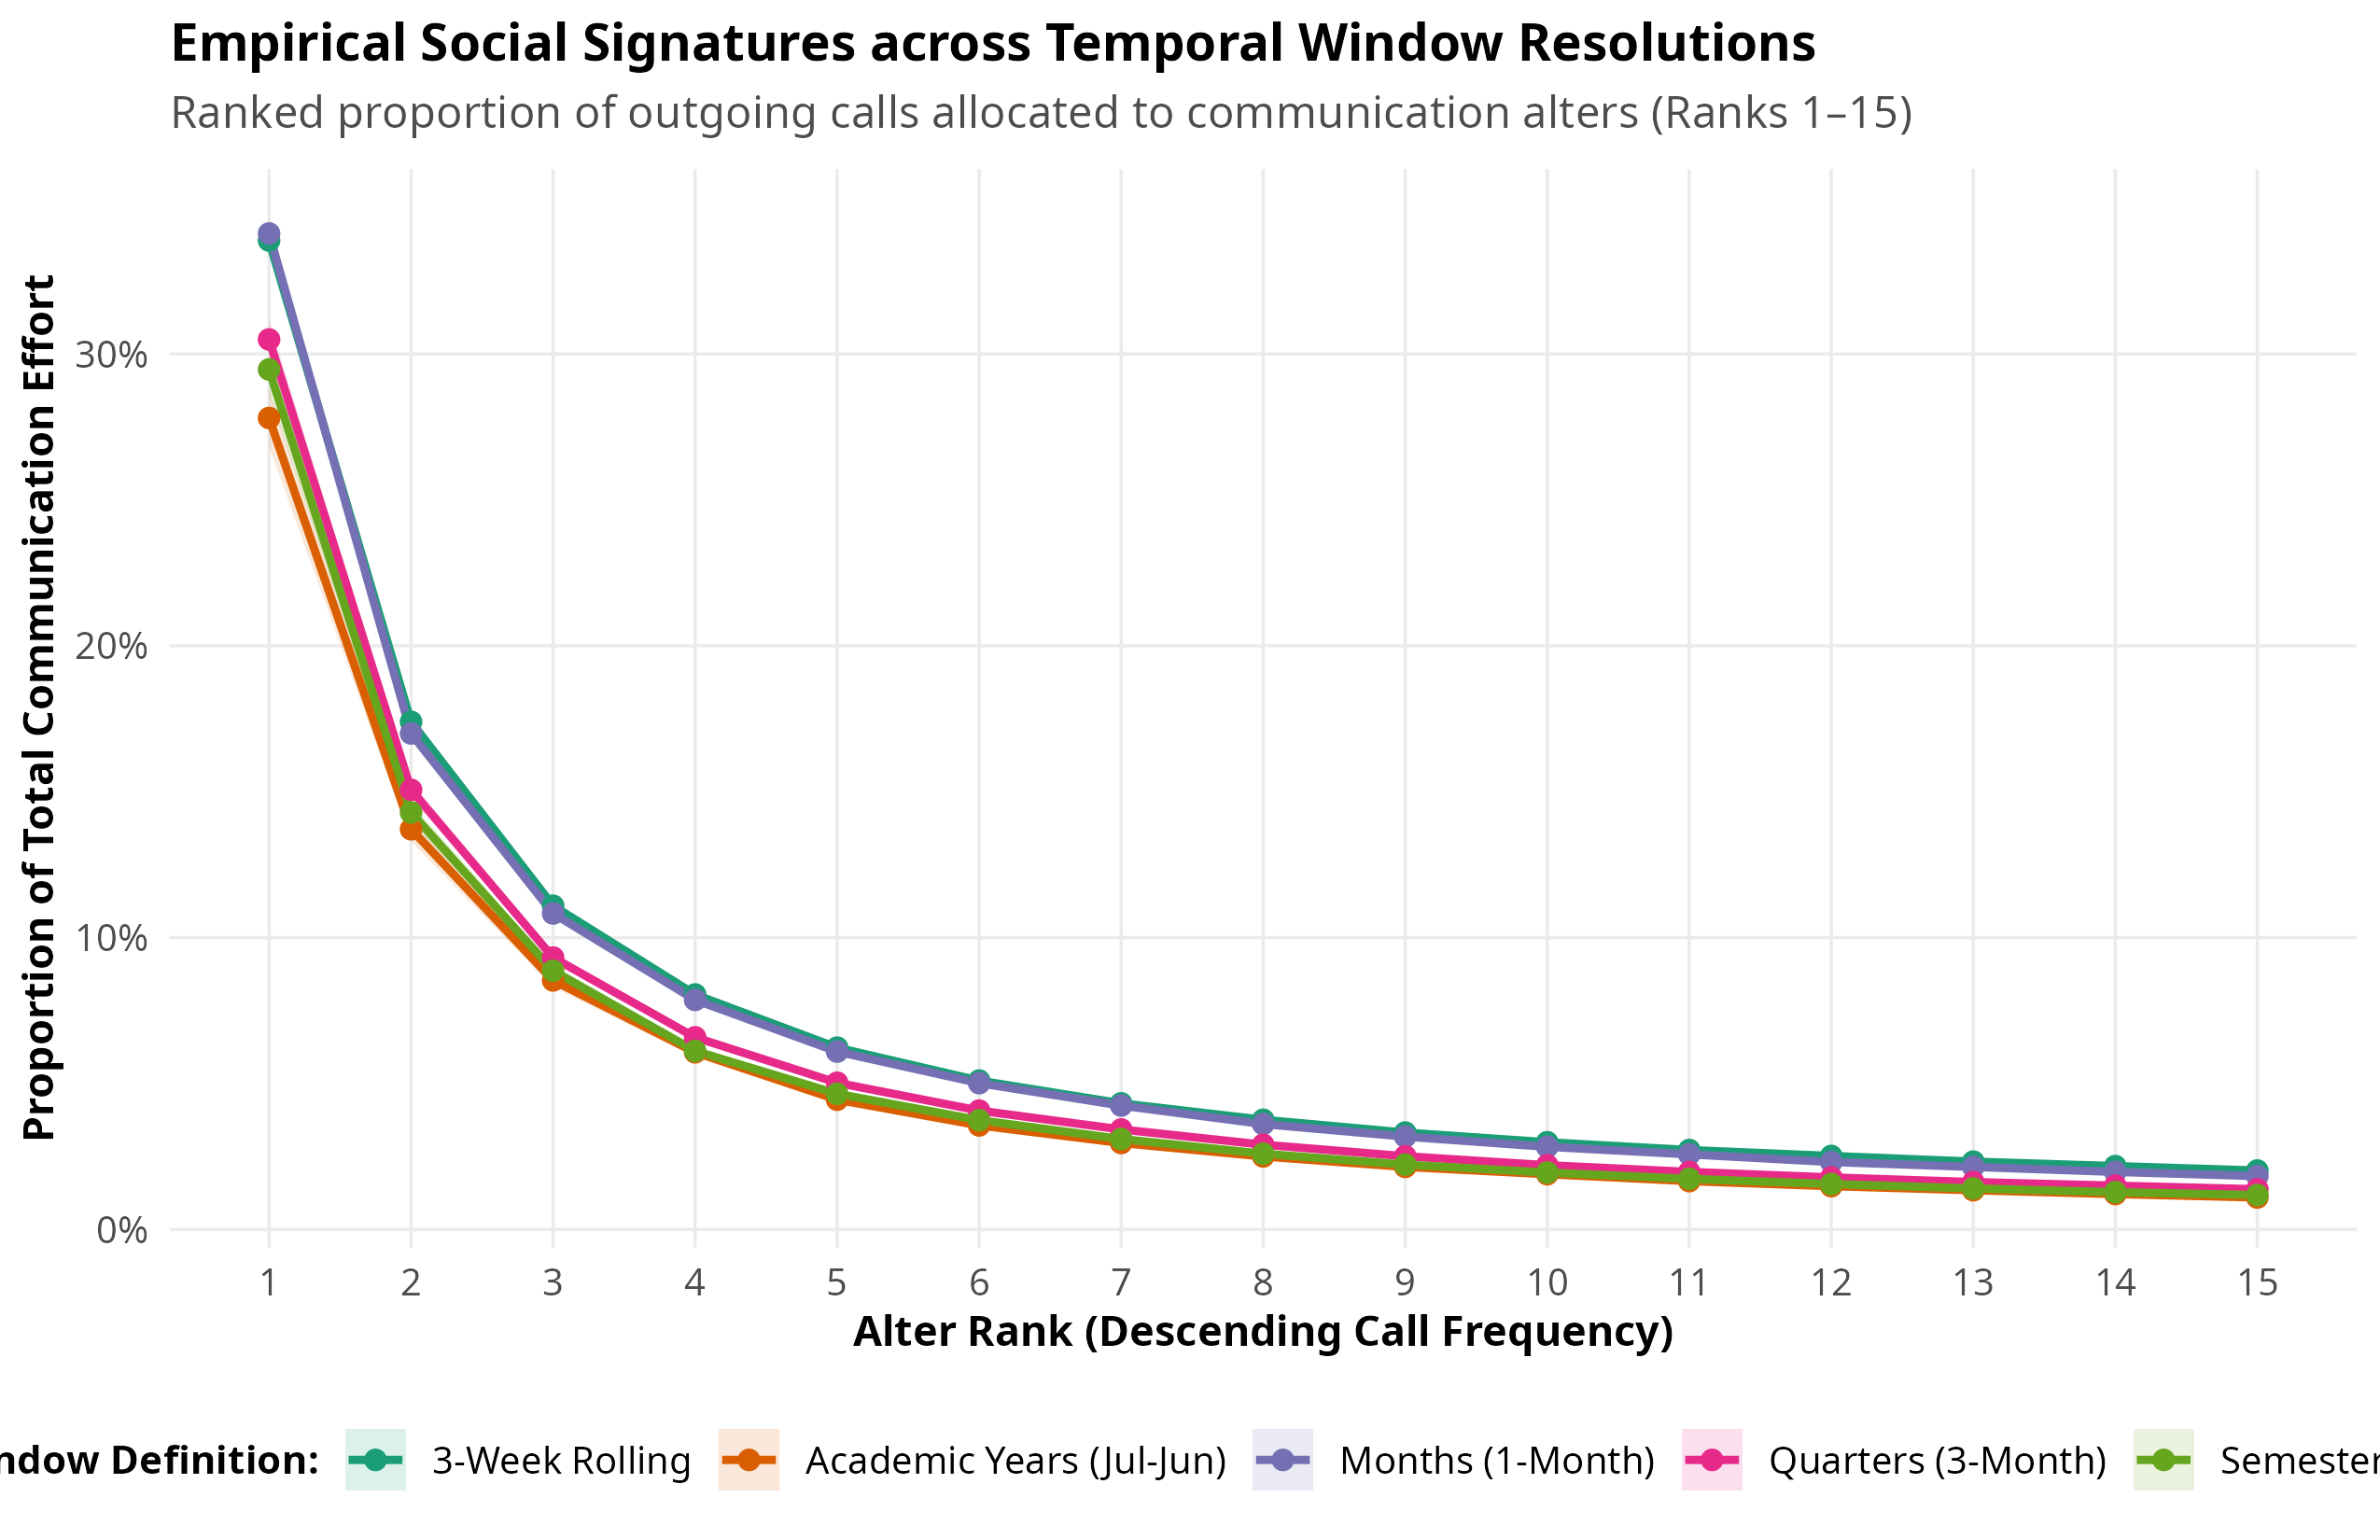
\includegraphics[width=0.88\textwidth]{Plots/fig01_mean_signatures_by_window.png}
\caption{\textbf{Empirical Social Signatures across Temporal Window Resolutions (Ranks 1--15).} Curves plot the mean proportion of outgoing communication directed to each alter rank across eight temporal window schemes (academic years, collegiate semesters, academic quarters, calendar months, 3-week rolling windows, 2-week discrete windows, and 1-week discrete windows). Ribbons denote 95\% confidence intervals around the mean interaction proportion.}
\label{fig:mean_signatures}
\end{figure}

To determine whether individuals maintain stable allocation profiles over time, we compared intraindividual self-divergence ($\dself$, the mean pairwise Jensen-Shannon Divergence between consecutive windows for the same ego) against interindividual reference divergence ($\dref$, the divergence between distinct individuals in the same window). Across every temporal resolution examined, intraindividual self-divergence is systematically and significantly lower than interindividual reference divergence ($p < 0.0001$, Wilcoxon signed-rank test; Cohen's $d > 1.4$; Extended Data Table~\ref{tab:stability_tests}). 

In collegiate semester windows ($N = 290$), mean self-divergence is 0.0614 ($\text{SD} = 0.0423$), less than half the reference divergence observed between random peers ($\dref = 0.1184, \text{SD} = 0.0304; V = 1,136, p < 0.0001$). Even at fine-grained weekly scales (3-week rolling windows, $N = 88$), an individual's signature remains consistent across time ($\dself = 0.0495$) relative to the broader population ($\dref = 0.1411, p < 0.0001$). As shown in Figure~\ref{fig:self_vs_ref}, the distributions of self and reference divergence exhibit minimal overlap across all timescales, confirming that personal communication signatures represent enduring individual behavioral profiles rather than transient fluctuations.

\begin{figure}[htbp]
\centering
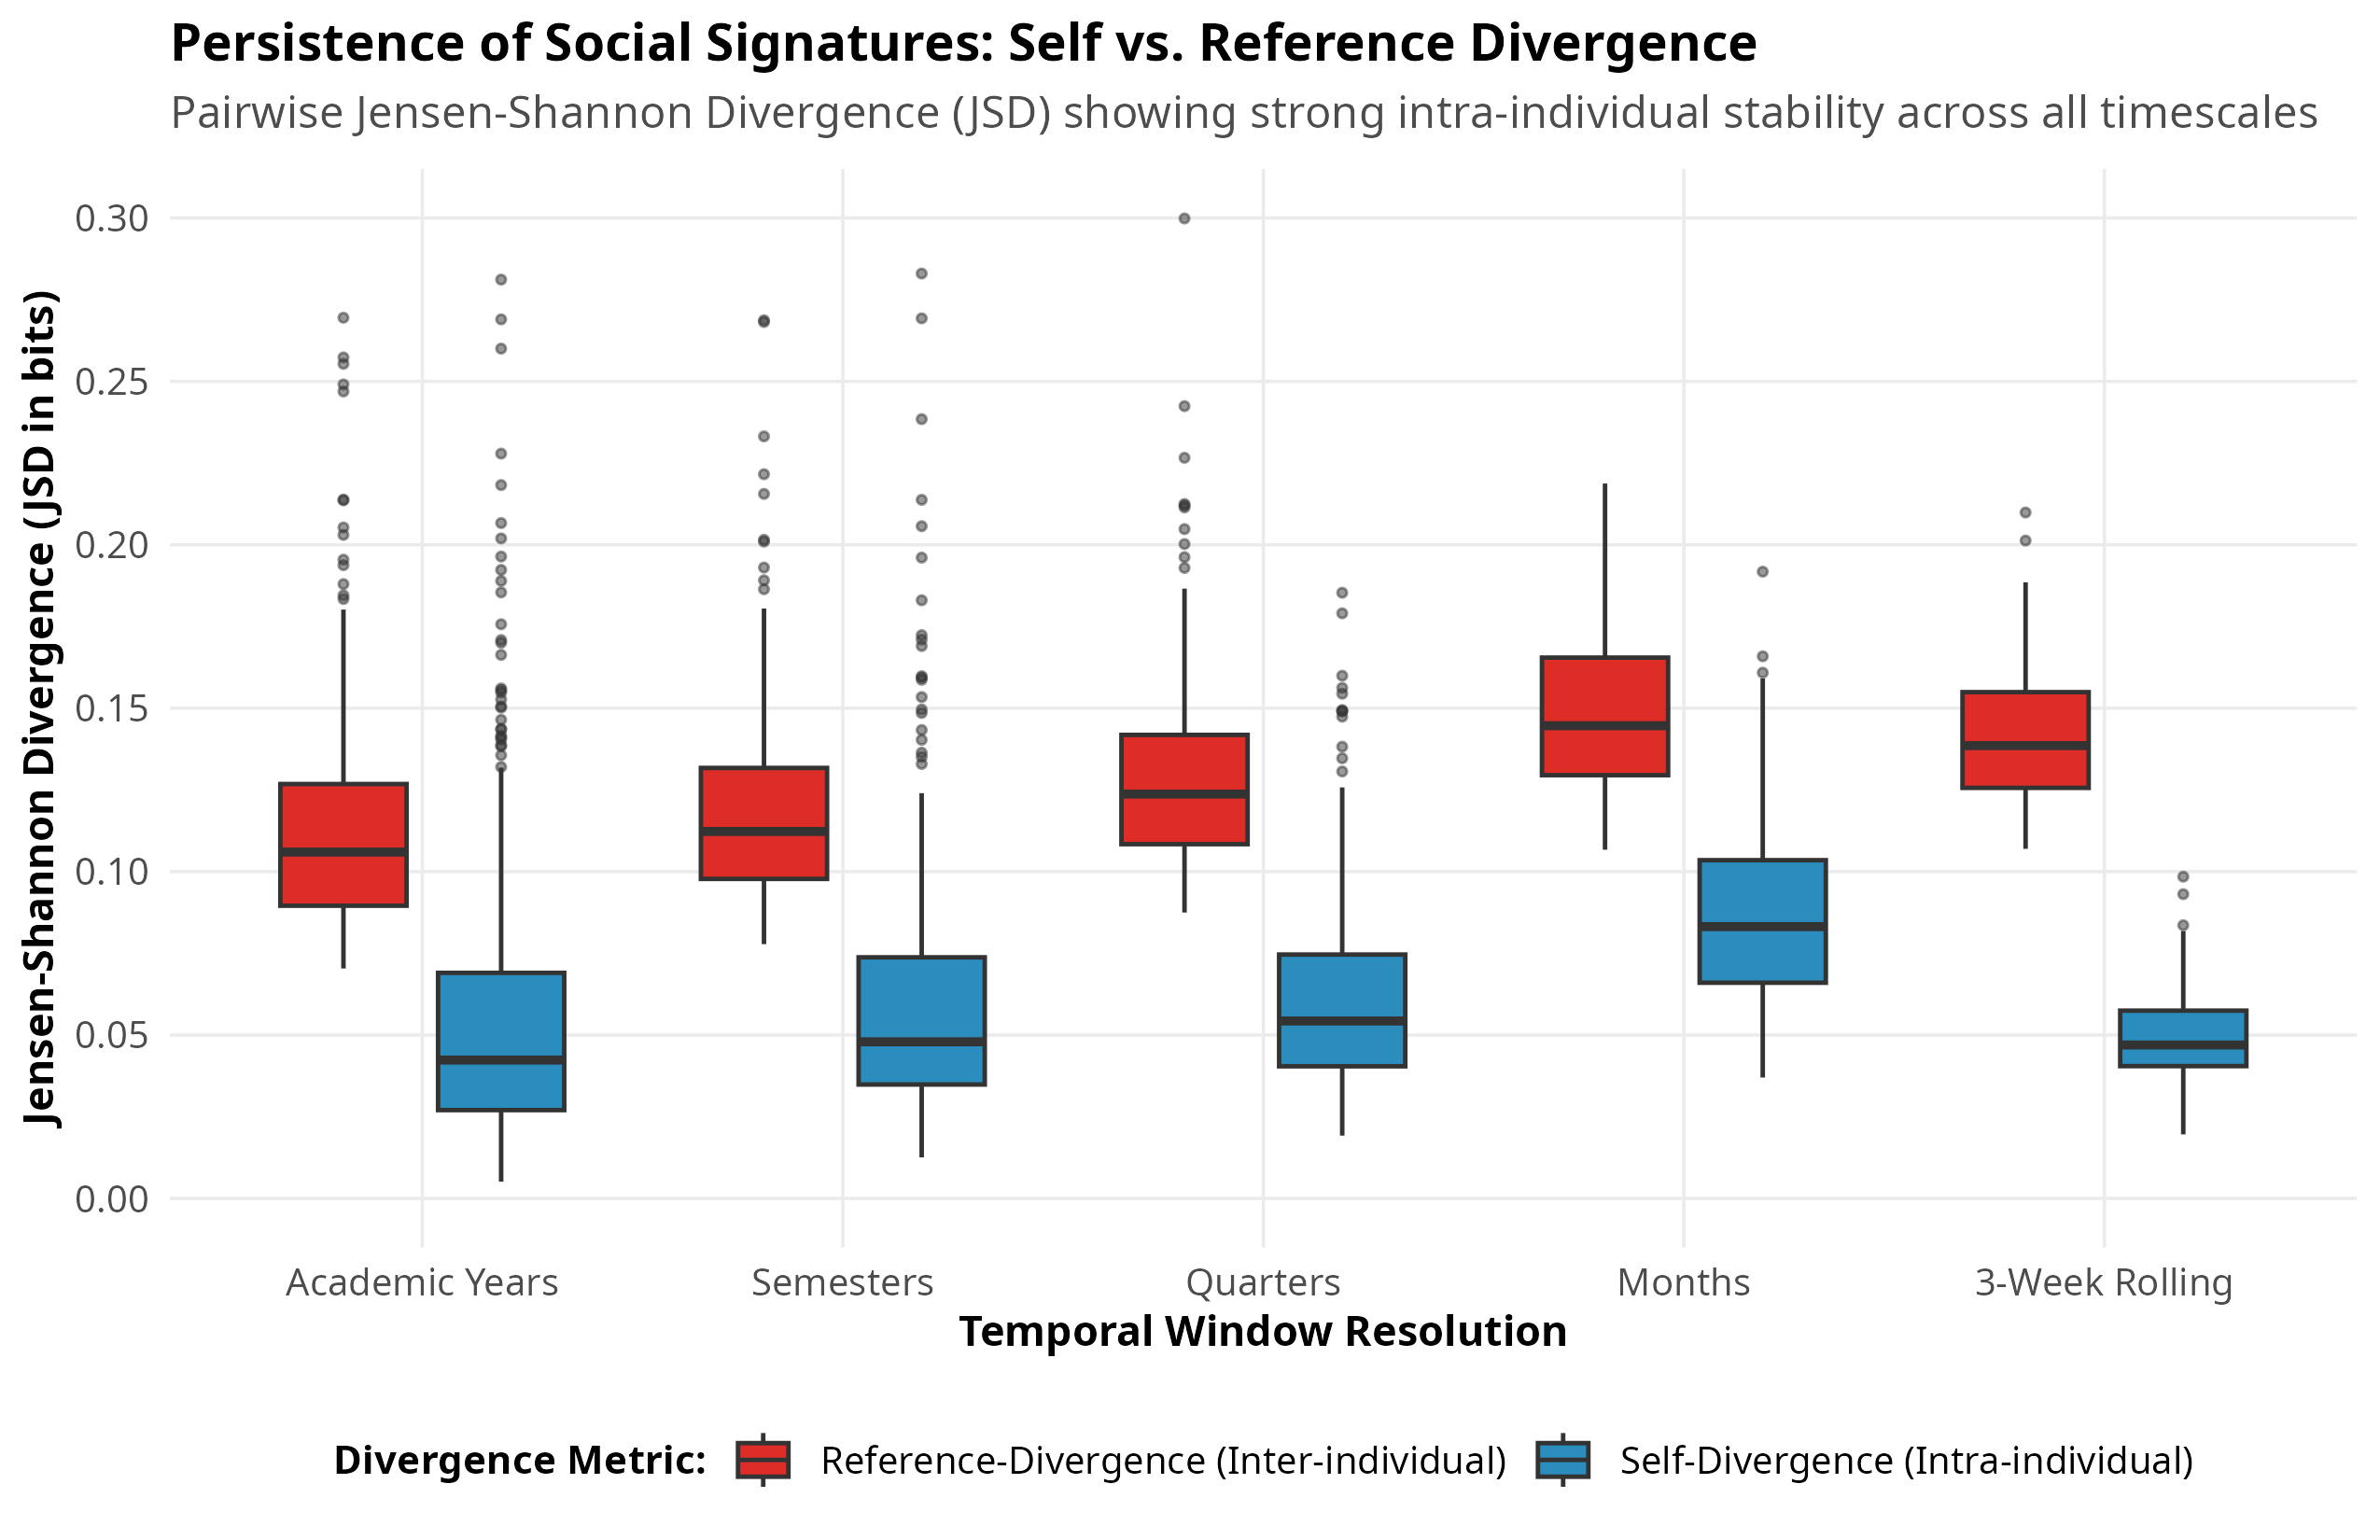
\includegraphics[width=0.88\textwidth]{Plots/fig02_self_vs_ref_divergence.png}
\caption{\textbf{Persistence of Social Signatures: Self-Divergence vs.\ Reference-Divergence across Temporal Resolutions.} Boxplots show the distribution of individual ego means for intraindividual self-divergence ($\dself$, blue) and interindividual reference divergence ($\dref$, orange) across eight temporal window schemes. Across all schemes, self-divergence is significantly lower than reference divergence ($p < 0.0001$, Wilcoxon signed-rank tests), demonstrating intraindividual signature stability.}
\label{fig:self_vs_ref}
\end{figure}

\subsection*{Parametric scaling and parameter burn-in convergence}

We next evaluated whether the continuous decay of communication effort is better described by a power-law decay specification ($p(r) = c \cdot r^{-\alpha}$) or an exponential decay model ($p(r) = c \cdot e^{-\beta r}$). Nonlinear least squares and log-linear regressions fit to each ego-window observation indicate that the power-law model decisively outperforms the exponential specification across both semester and monthly timescales (Figure~\ref{fig:power_law_exp} and Extended Data Table~\ref{tab:parametric_models}).

\begin{figure}[htbp]
\centering
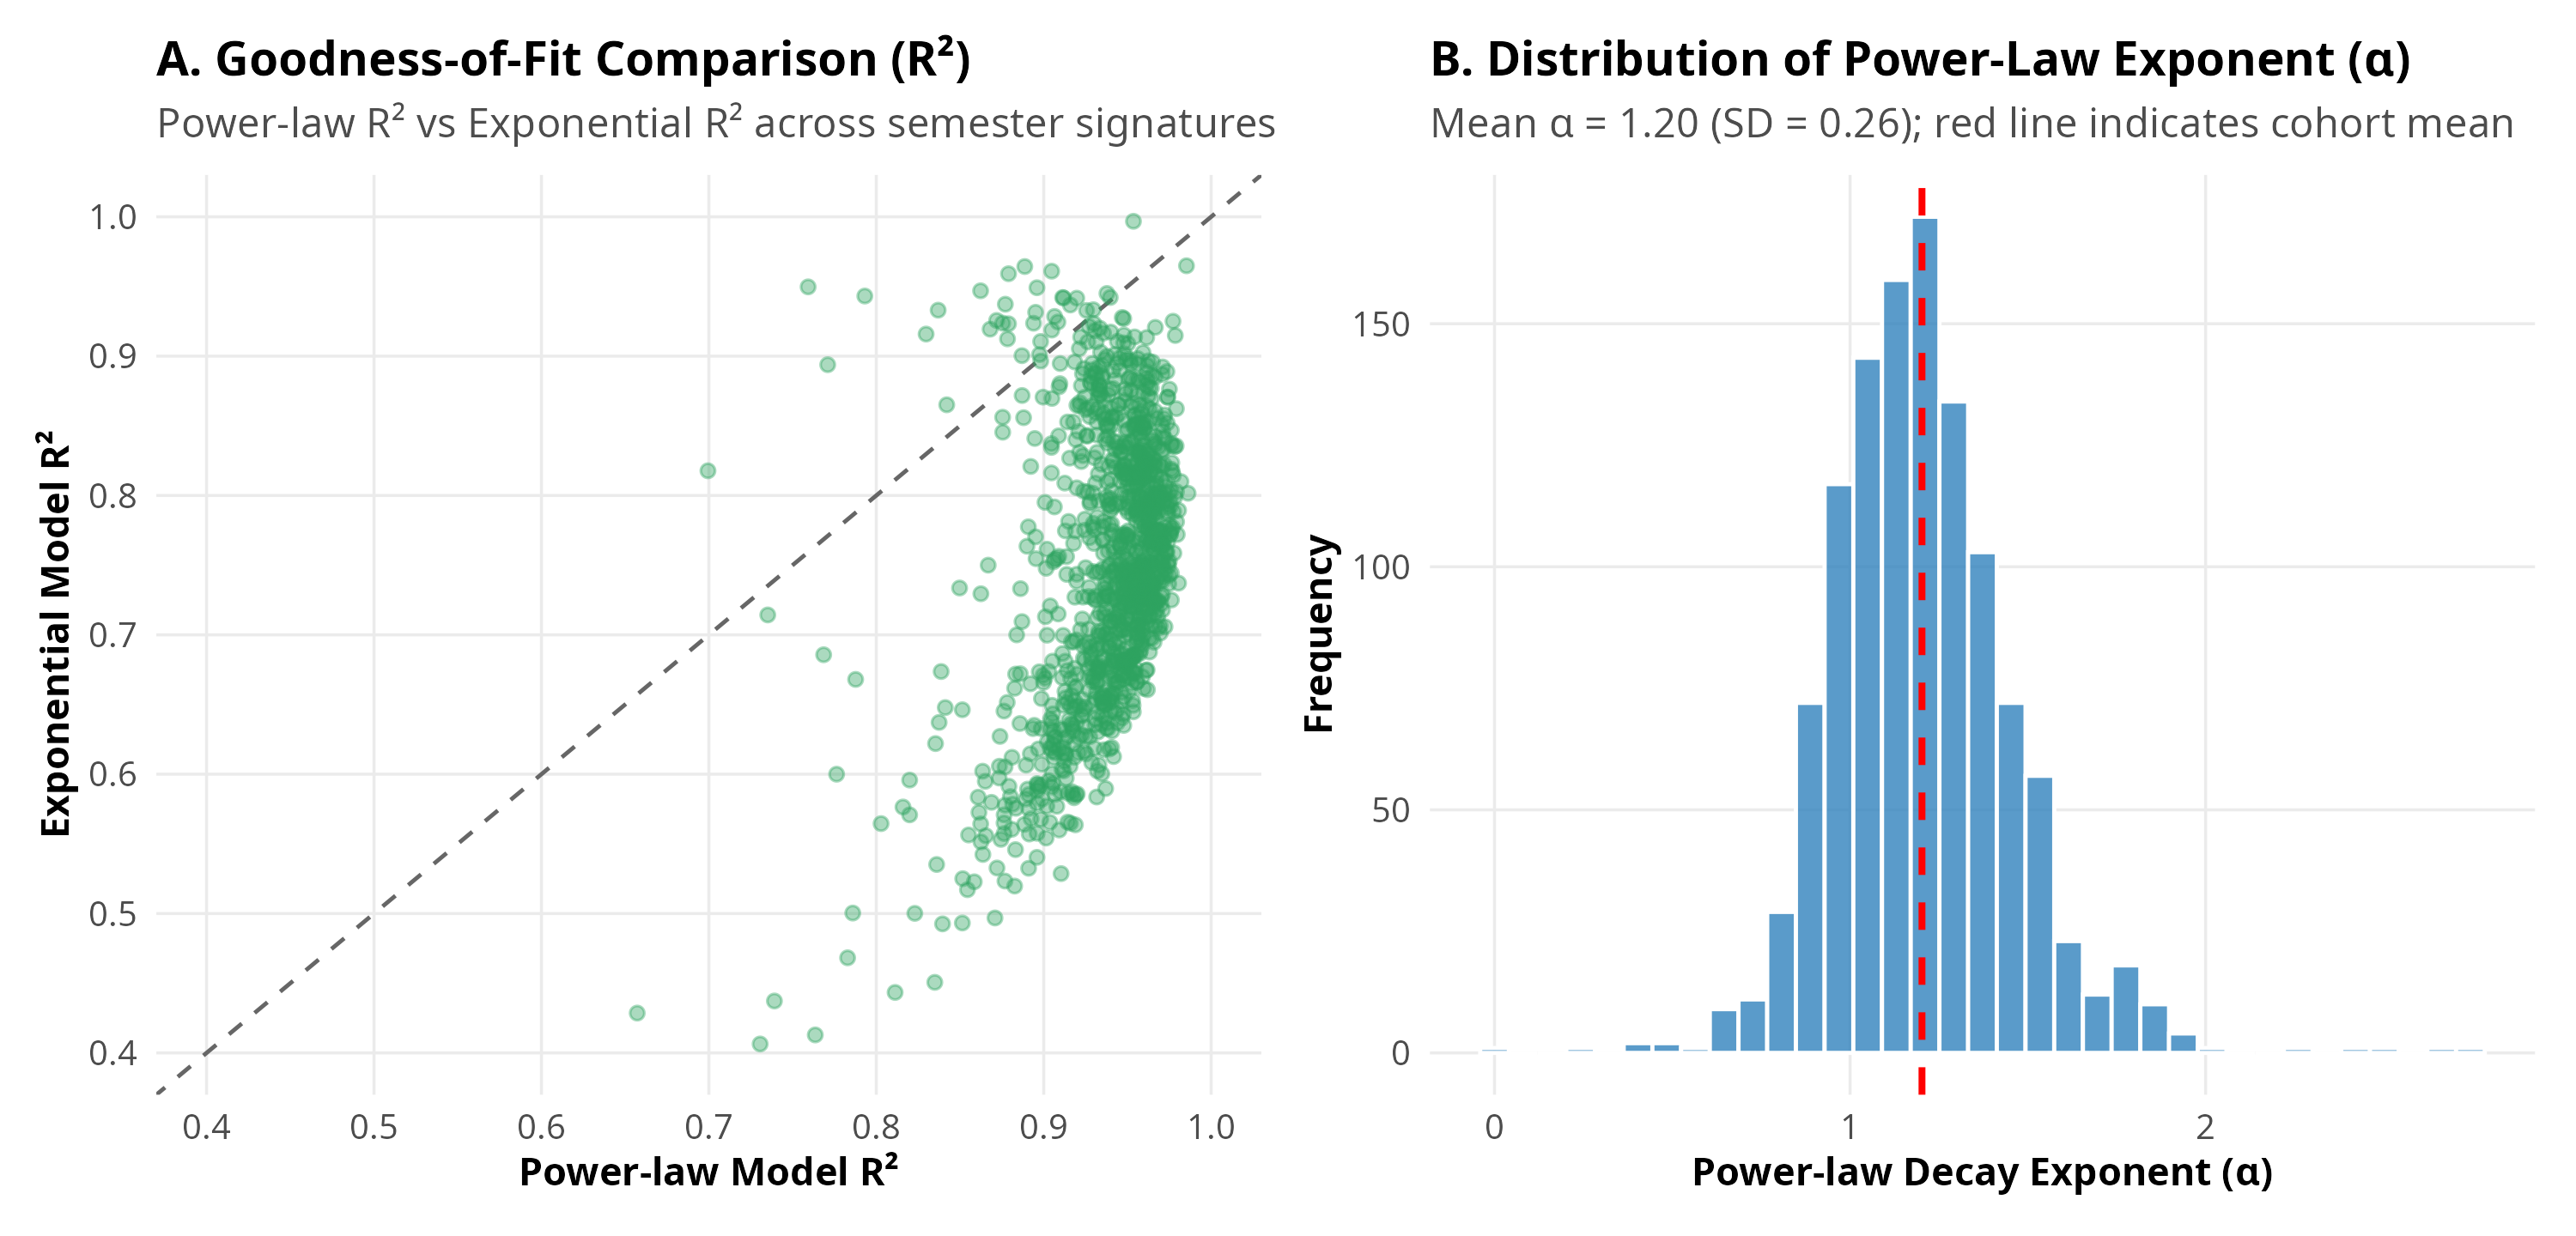
\includegraphics[width=0.92\textwidth]{Plots/fig03_power_law_vs_exponential.png}
\caption{\textbf{Parametric Power-Law vs.\ Exponential Model Fits and Exponent Distribution.} \textbf{a}, Scatterplot of coefficient of determination ($R^2$) values comparing power-law against exponential fits across semester signatures ($N = 1,158$ models); points above the diagonal indicate superior fit for the power-law specification. \textbf{b}, Empirical probability density distribution of the estimated power-law decay exponent ($\alpha$), showing an average exponent of $\bar{\alpha} = 1.20$ ($\text{SD} = 0.26$).}
\label{fig:power_law_exp}
\end{figure}

In semester windows ($N = 1,158$ models), the power-law specification is preferred by Akaike's Information Criterion (AIC) in 97.0\% of models, yielding an average $R^2$ of 0.935 (compared to 0.746 for exponential decay; Figure~\ref{fig:power_law_exp}a). The estimated power-law decay exponent $\alpha$ averages 1.20 ($\text{SD} = 0.26$; Figure~\ref{fig:power_law_exp}b), reflecting a heavy-tailed allocation profile. In monthly windows ($N = 3,496$ models), the power-law model remains preferred in 83.8\% of cases (mean $R^2 = 0.883$ vs.\ 0.771).

A critical question for network sensing research is parameter burn-in: how long must an individual be continuously observed before their estimated signature parameters stabilize? Tracking the common cohort ($N = 147$) across cumulative observation windows from 2 to 24 months shows that parameter estimates stabilize asymptotically within six to eight months of continuous digital observation (Extended Data Fig.~\ref{fig:burnin}). At two months, the mean absolute error is 0.188 relative to the 24-month benchmark; by six months, mean absolute error drops below 0.10 ($R^2 = 0.945$). This establishes an empirical burn-in guideline for observational study designs.

\subsection*{Role relations and dimensions of social support across signature ranks}

To resolve the content black box of digital communication logs, we matched the calling records of the collegiate semester cohort ($N = 290$ egos) to longitudinal ego-network surveys recording relationship categories and dimensions of social support. This linkage matched $N = 13,174$ call-ranked dyadic observations across 283 unique egos (7 egos nominated no active alters in the survey) to six theoretical Dunbar tiers (Table~\ref{tab:support_tiers} and Figure~\ref{fig:support_tiers}).

\begin{table}[htbp]
\centering
\caption{\textbf{Relational Composition and Support Functions Across Signature Rank Tiers ($N = 13,174$ Dyads)}}
\label{tab:support_tiers}
\small
\resizebox{\textwidth}{!}{%
\begin{tabular}{lccccccc}
\toprule
\textbf{Rank Tier} & \textbf{Ties ($N$)} & \textbf{\% Family} & \textbf{\% Friend} & \textbf{\% Emotional} & \textbf{\% Advice} & \textbf{\% Companionship} & \textbf{\% Financial} \\
\midrule
Rank 1 (Core) & 950 & 69.7\% & 16.9\% & 85.4\% & 87.6\% & 80.6\% & 64.1\% \\
Ranks 2--3 & 1,713 & 62.2\% & 34.0\% & 77.1\% & 80.1\% & 79.8\% & 45.1\% \\
Ranks 4--5 & 1,426 & 41.4\% & 56.9\% & 70.0\% & 73.0\% & 81.9\% & 24.2\% \\
Ranks 6--10 & 2,743 & 24.2\% & 74.4\% & 60.7\% & 64.3\% & 78.2\% & 12.4\% \\
Ranks 11--20 & 3,011 & 14.3\% & 84.5\% & 48.1\% & 53.6\% & 74.4\% & 7.1\% \\
Ranks $>20$ & 3,331 & 9.2\% & 87.8\% & 39.1\% & 44.0\% & 69.5\% & 4.4\% \\
\bottomrule
\multicolumn{8}{l}{\footnotesize Tie counts represent unique call-ranked dyad-window observations linked to ego-network surveys.}
\end{tabular}%
}
\end{table}

These patterns uncover three fundamental regularities. First, the kinship core at Rank 1 is heavily dominated by family members (69.7\% kin, primarily parents and romantic partners), who provide the structural foundation of instrumental, advisory, and financial assistance (64.1\% financial aid, 87.6\% advice, and 85.4\% emotional support). Second, a structural friendship transition occurs between Ranks 3 and 5: while family members still constitute 62.2\% of ties at Ranks 2--3, peer friends constitute the majority (56.9\%) by Ranks 4--5, rising to 87.8\% beyond Rank 20 (Figure~\ref{fig:support_tiers}a). Third, the data reveal a differentiated support gradient across tiers (Figure~\ref{fig:support_tiers}b): while emotional support (85.4\% at Rank 1) and advice support (87.6\% at Rank 1) fall monotonically across tiers (dropping to 39.1\% and 44.0\% for outer ties), companionship remains elevated across all tiers (80.6\% at Rank 1, 81.9\% at Ranks 4--5, and 69.5\% beyond Rank 20). This demonstrates that peripheral communication ties serve vital leisure, recreation, and social integration functions rather than representing casual acquaintances.

\begin{figure}[htbp]
\centering
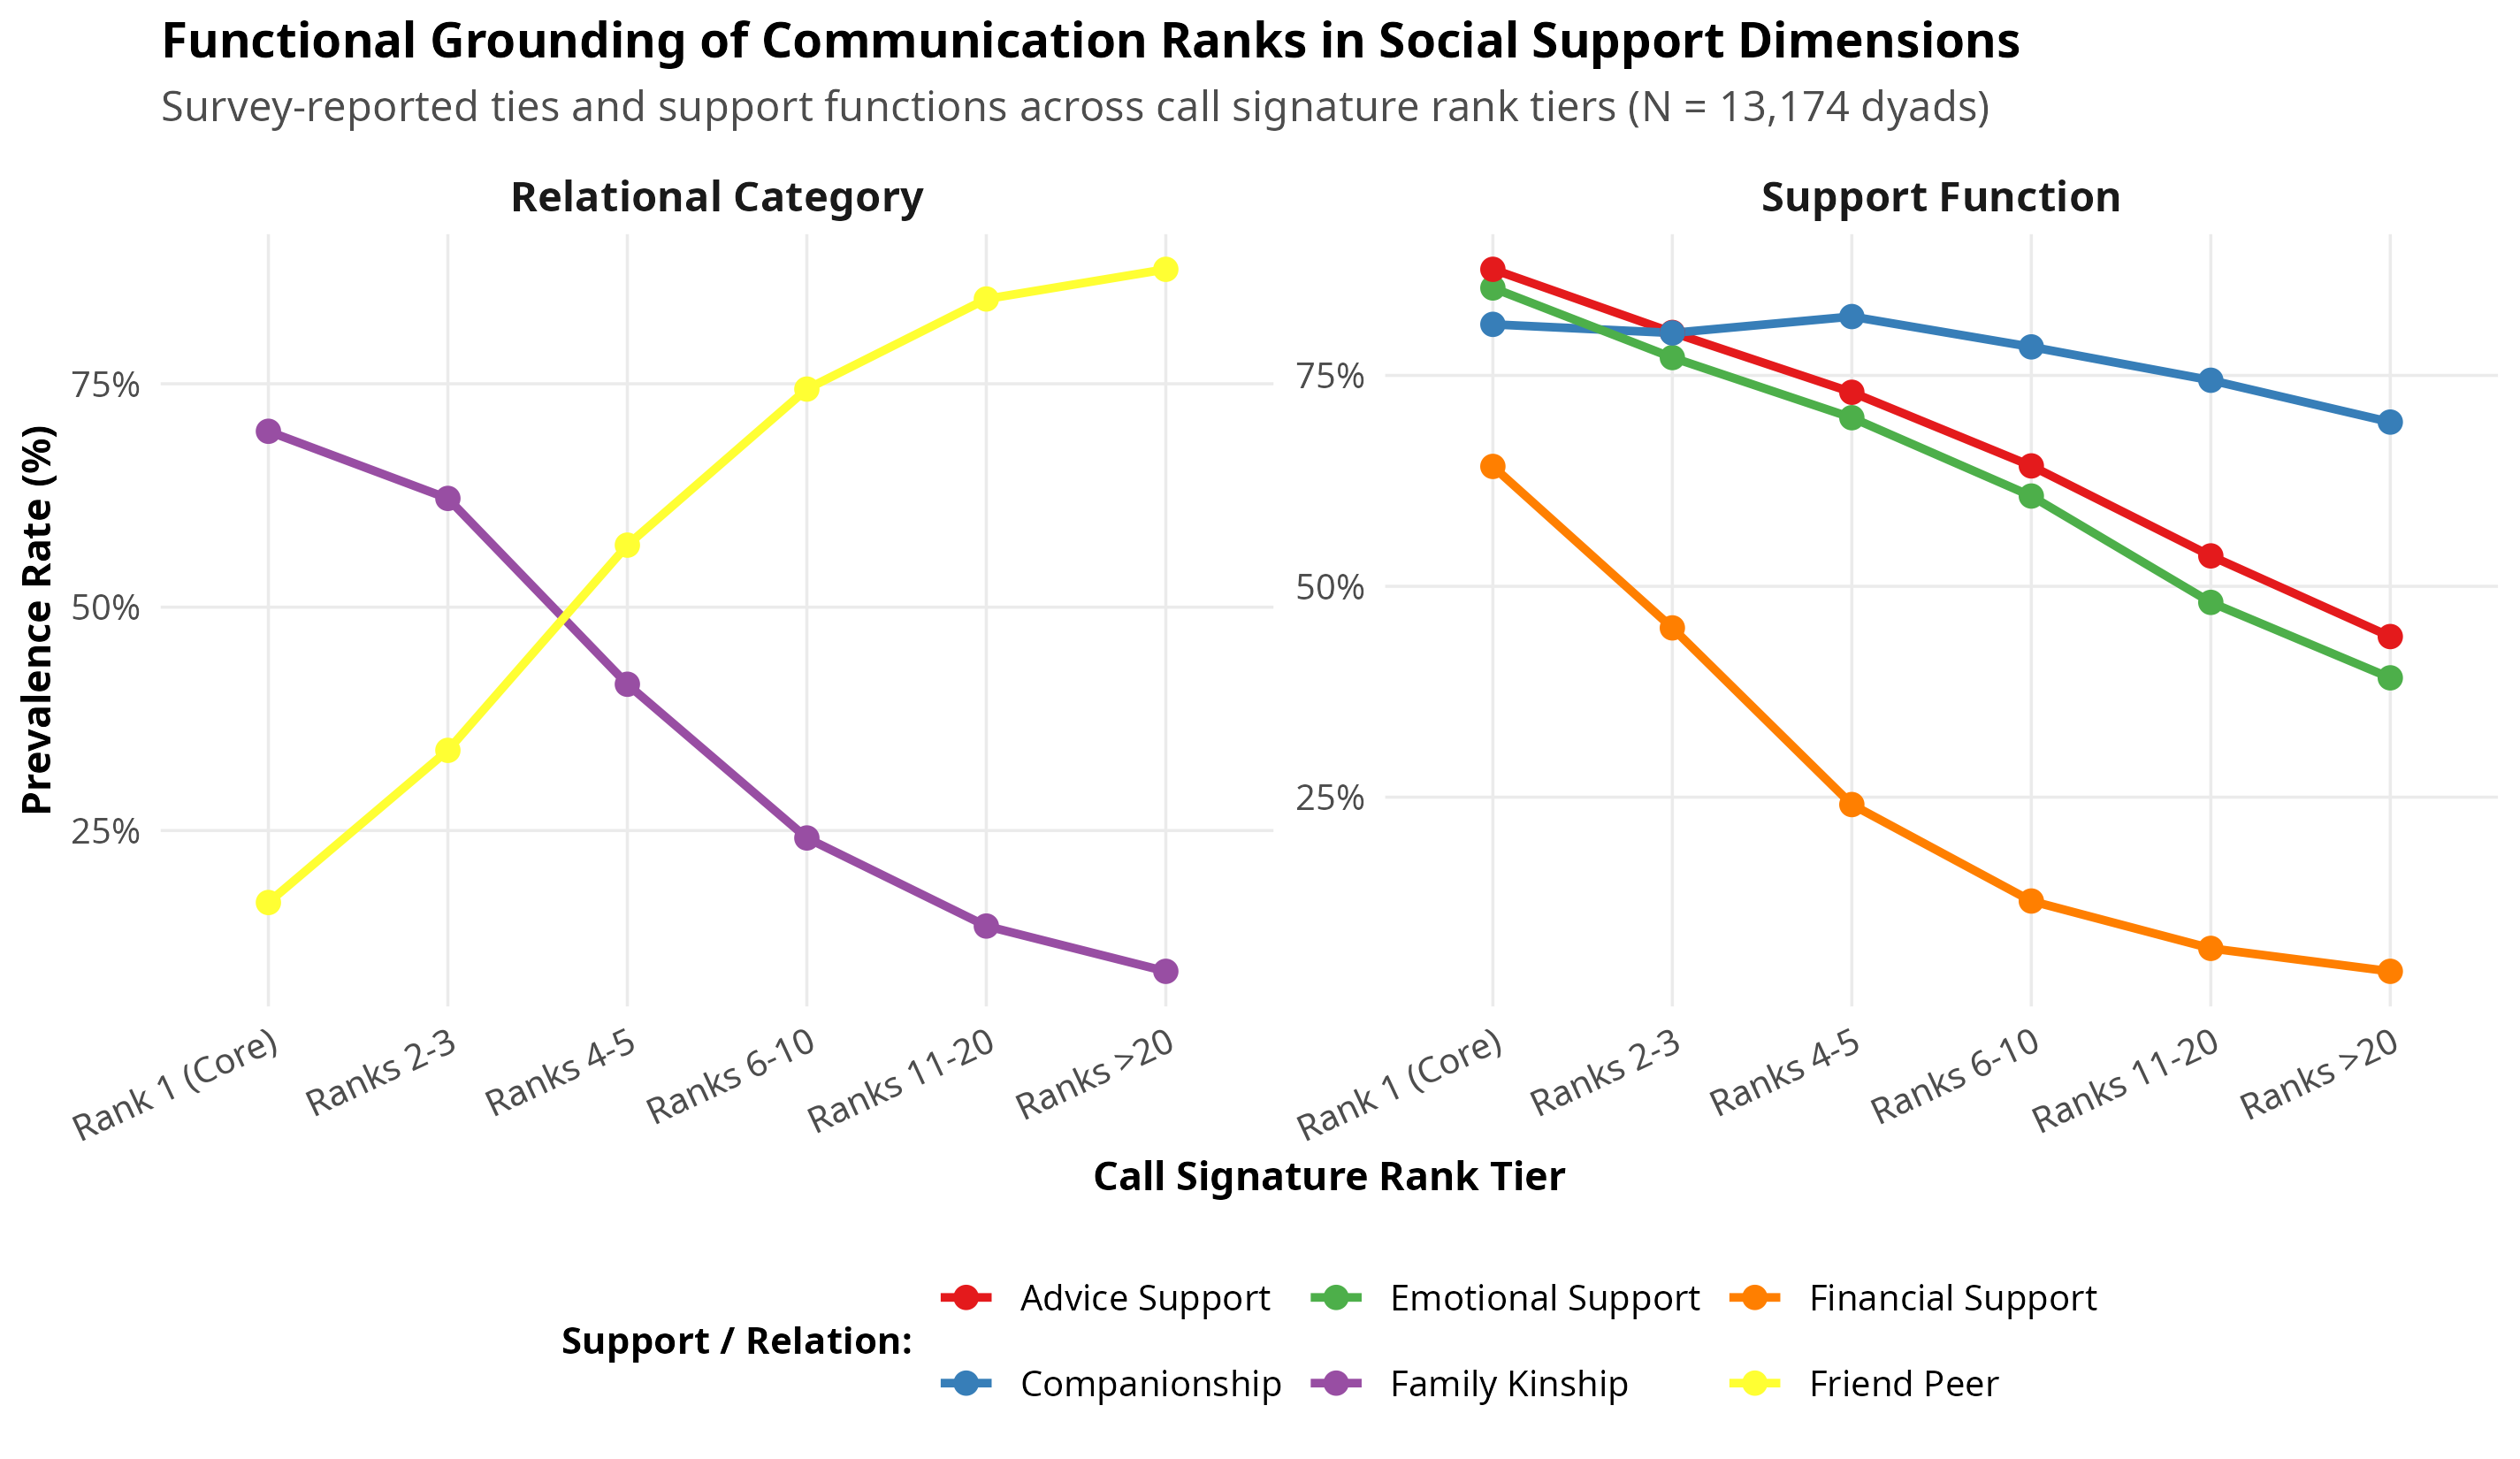
\includegraphics[width=0.92\textwidth]{Plots/fig05_rank_by_support_tiers.png}
\caption{\textbf{Dimensions of Social Support Across Signature Rank Tiers ($N = 13,174$ Dyads).} \textbf{a}, Proportion of ties categorized as family kin versus peer friends across six signature rank tiers, showing the structural transition from kinship dominance at Ranks 1--3 to peer friendship dominance at Ranks 4 and above. \textbf{b}, Prevalence of specific social support provisions (emotional comfort, advice/guidance, social companionship, and financial aid) across signature tiers.}
\label{fig:support_tiers}
\end{figure}

\subsection*{Evaluative and cognitive alignment of communication slots}

Beyond categorical support provisions, an alter's signature position slot strongly aligns with evaluative and cognitive dimensions of the tie (Extended Data Fig.~\ref{fig:tie_evaluative}). Subjective closeness\cite{marsden1984measuring-f62} exhibits a steep monotonic gradient across signature tiers ($F = 280.1, p < 0.0001$): 93.7\% of alters in the Rank 1 slot are rated as ``especially close'' (mean rating 3.93 on a 1--4 scale), declining to 78.5\% at Ranks 4--5 and 52.7\% at Ranks $>20$ ($r = -0.222, p < 0.0001$). Relationship duration\cite{burt2000decay-f08} displays an even sharper sorting ($F = 581.0, p < 0.0001$): Rank 1 alters average 14.2 years of acquaintance (median 18.8 years), capturing lifelong kin, whereas intermediate tiers average 7.0 years and outer tiers average 4.9 years ($r = -0.266, p < 0.0001$). Furthermore, signature rank corresponds closely to cognitive recall salience ($F = 334.0, p < 0.0001$): 71.2\% of Rank 1 alters are recalled within the first 5 alters named in surveys (36.4\% named first), whereas outer alters average a recall position of 9.9 ($r = +0.243, p < 0.0001$).

\begin{table}[htbp]
\centering
\caption{\textbf{Linear Mixed-Effects Models Predicting Signature Allocation and Rank from Tie Attributes ($N = 10,828$ Dyads across 280 Egos)}}
\label{tab:tie_regressions}
\small
\resizebox{\textwidth}{!}{%
\begin{tabular}{lcccc}
\toprule
\textbf{Predictor Term} & \textbf{Model 1 (Evaluative)} & \textbf{Model 2 (+ Duration)} & \textbf{Model 3 (+ Salience)} & \textbf{Model 4 (Full Rank)} \\
\midrule
Intercept & $-0.1787^{***}\ (0.0078)$ & $-0.1243^{***}\ (0.0077)$ & $-0.1417^{***}\ (0.0074)$ & $47.0176^{***}\ (1.3673)$ \\
Subjective Closeness (1--4) & $0.0374^{***}\ (0.0025)$ & $0.0274^{***}\ (0.0024)$ & $0.0115^{***}\ (0.0024)$ & $-4.2135^{***}\ (0.4423)$ \\
Interpersonal Trust (1--10) & $0.0122^{***}\ (0.0008)$ & $0.0071^{***}\ (0.0008)$ & $0.0056^{***}\ (0.0008)$ & $-0.1429\ (0.1466)$ \\
Tie Duration (Years) & -- & $0.0034^{***}\ (0.0001)$ & $0.0035^{***}\ (0.0001)$ & $-0.4804^{***}\ (0.0212)$ \\
Cognitive Salience ($26 - \text{Order}$) & -- & -- & $0.0047^{***}\ (0.0002)$ & $-0.6922^{***}\ (0.0363)$ \\
\midrule
Dependent Variable & Call Proportion ($p$) & Call Proportion ($p$) & Call Proportion ($p$) & Signature Rank ($r$) \\
Dyadic Observations & 10,828 & 10,828 & 10,828 & 10,828 \\
Ego Clusters ($J$) & 280 & 280 & 280 & 280 \\
Ego Random Variance ($\tau_{00}$) & 0.00092 & 0.00061 & 0.00042 & 24.49 \\
Residual Variance ($\sigma^2$) & 0.00752 & 0.00707 & 0.00678 & 217.10 \\
Intraclass Correlation (ICC) & 0.109 & 0.079 & 0.058 & 0.101 \\
\bottomrule
\multicolumn{5}{l}{\footnotesize Standard errors in parentheses. $^{***}p < 0.0001$, $^{**}p < 0.01$, $^*p < 0.05$.}
\end{tabular}%
}
\end{table}

Because ties are nested within egos ($N = 10,828$ complete dyads across $J = 280$ individuals, averaging 38.7 ties per ego), we estimated linear mixed-effects models with ego random intercepts (Table~\ref{tab:tie_regressions}). In Model~1, the ego-level intraclass correlation is 0.109, indicating that roughly 11\% of the variance in communication allocation is attributable to individual-level baselines. Subjective closeness ($t = 15.07, p < 0.0001$) and interpersonal trust ($t = 14.41, p < 0.0001$) strongly predict call proportion. Adding tie duration in Model~2 confirms that relationship longevity exerts a powerful independent effect ($t = 27.95, p < 0.0001$). Model~3 shows that cognitive salience further drives communication ($t = 23.47, p < 0.0001$), while duration ($t = 30.26$), closeness ($t = 4.73$), and trust ($t = 6.95$) each retain highly significant positive effects. Finally, Model~4 shows that these attributes jointly govern an alter's ordinal signature rank ($p < 0.0001$), with greater closeness, longevity, and recall accessibility pulling alters closer to Rank~1.

\subsection*{Direct verification of the slot-filling mechanism}

A central theoretical puzzle in social signatures research is how personal allocation curves can remain stable despite substantial turnover in alter membership. We calculated dyadic Jaccard turnover between consecutive semesters:
\begin{equation}
\Turnover_{i,w} = 1 - \frac{|A_{i,w} \cap A_{i,w+1}|}{|A_{i,w} \cup A_{i,w+1}|}
\end{equation}
where $A_{i,w}$ denotes the active alter set for ego $i$ in window $w$.

\begin{figure}[htbp]
\centering
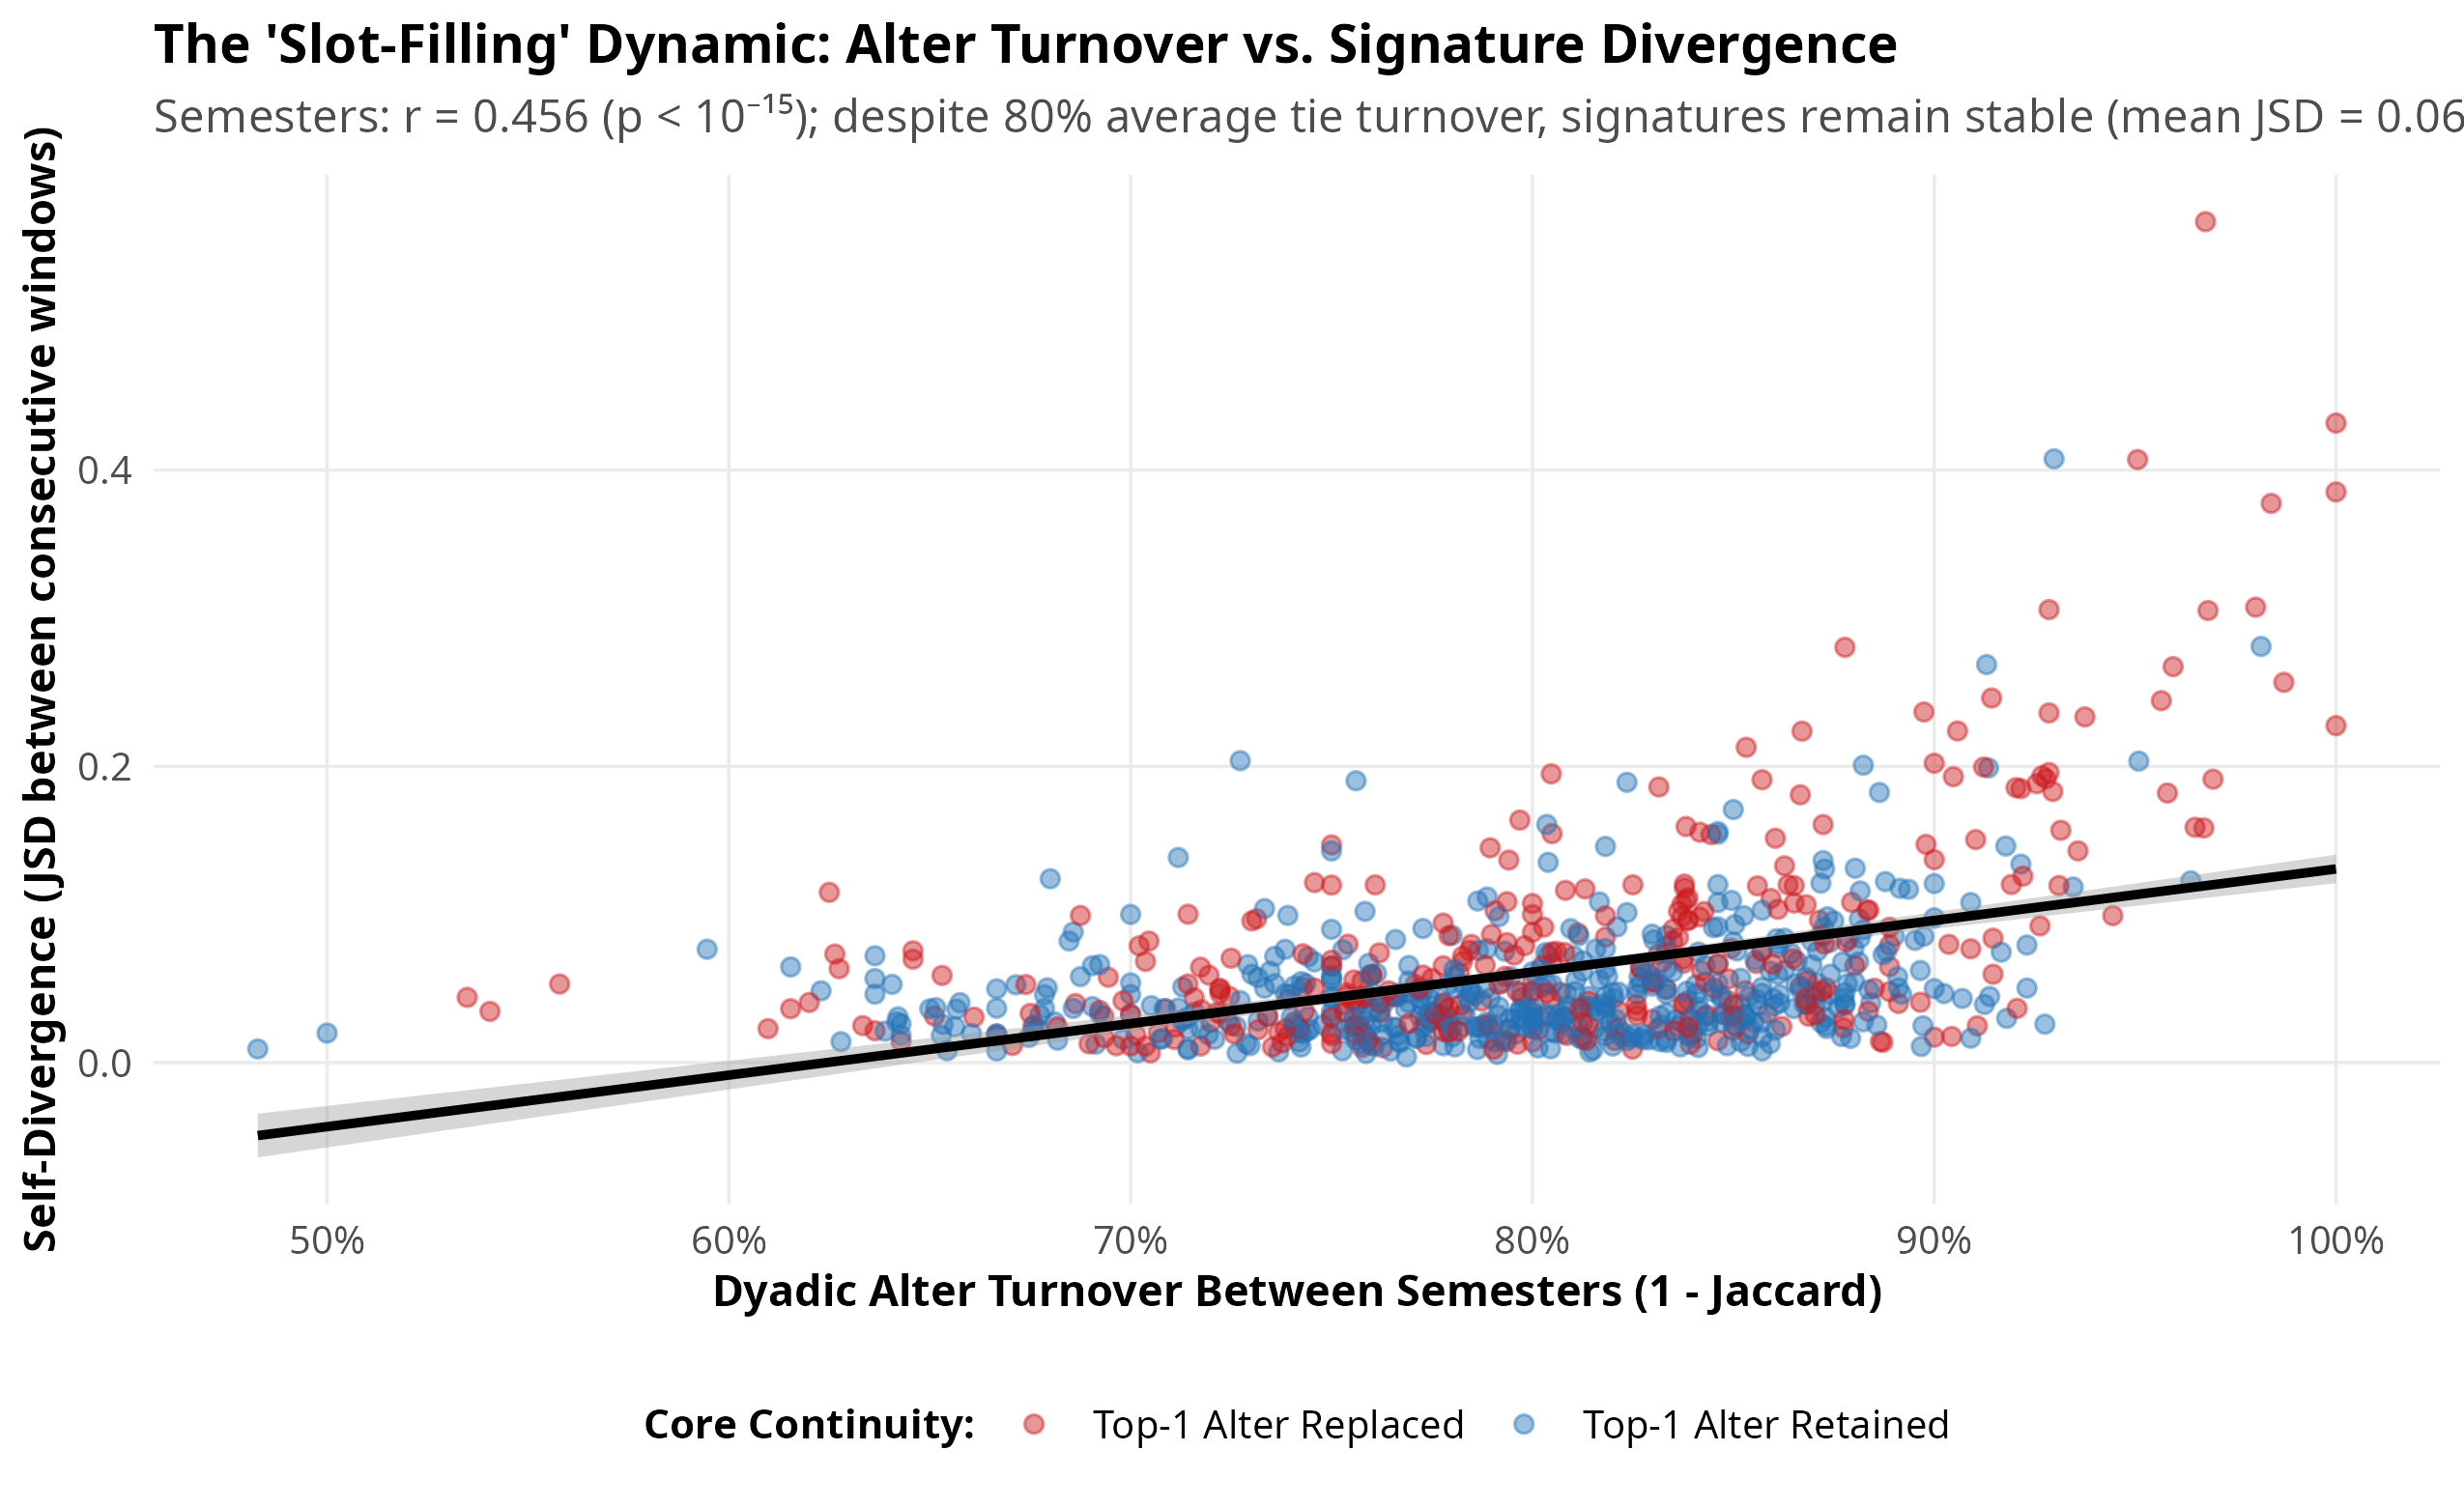
\includegraphics[width=0.88\textwidth]{Plots/fig06_turnover_vs_stability.png}
\caption{\textbf{The `Slot-Filling' Dynamic: Alter Turnover vs.\ Signature Divergence ($r = 0.456, p < 0.0001$).} Scatterplot shows dyadic Jaccard alter turnover against Jensen-Shannon self-divergence ($\dself$) across consecutive semesters ($N = 870$ transitions across 290 egos). Blue points denote transitions where the Rank 1 alter was retained (mean $\dself = 0.0431$); red points denote transitions where the Rank 1 alter was replaced (mean $\dself = 0.0785$).}
\label{fig:turnover}
\end{figure}

Alter turnover between consecutive semesters averages 80.1\% ($\text{SD} = 0.076$). Despite replacing four out of five alters every six months, egos preserve signature stability ($\dself = 0.0614$). In 59.1\% of consecutive semester intervals, the single top-ranked alter was retained (Figure~\ref{fig:turnover}, blue points; mean $\dself = 0.0431$). Crucially, even when the primary confidant was completely replaced by a new entrant (Figure~\ref{fig:turnover}, red points), self-divergence increased only modestly from 0.0431 to 0.0785. This pattern provides direct empirical verification of the \textit{slot-filling hypothesis}: individuals maintain a pre-existing relational architecture and slot newly acquired contacts into vacated functional positions without restructuring their overall allocation profile.

\subsection*{Multilevel panel dynamics of signature self-divergence}

To identify the structural drivers of signature divergence over time, we estimated linear mixed-effects panel models with ego random intercepts predicting $\JSD_{it}$ across consecutive semesters ($N = 870$ transitions across 290 egos; Extended Data Table~\ref{tab:multilevel_models}). Alter turnover is the primary driver of temporal variation in self-divergence ($\beta = 0.351, p < 0.0001$), accompanied by large shifts in communication volume ($\beta = 0.0014, p < 0.0001$). In contrast, ego network clustering ($\beta = -0.0066, p = 0.665$) and network density exert negligible effects net of turnover. This confirms that signature stability is governed by person-level allocation dynamics rather than the triadic closure of the surrounding peer network.

\subsection*{Personality determinants and non-linear buffering of signature curvature}

What psychological dispositions generate steep (core-concentrated) versus flat (diffuse) social signatures? Regressing ego-mean power-law decay exponents ($\alpha_i$) on Big Five personality traits and network degree ($N = 290$ egos; Extended Data Table~\ref{tab:personality_models}) reveals that Negative Emotionality strongly predicts signature steepness ($\beta = 0.098, t = 5.08, p < 0.0001$). Individuals higher in baseline Negative Emotionality exhibit systematically steeper decay exponents, funneling a larger proportion of their communication into one or two primary alters (Figure~\ref{fig:personality}a).

\begin{figure}[htbp]
\centering
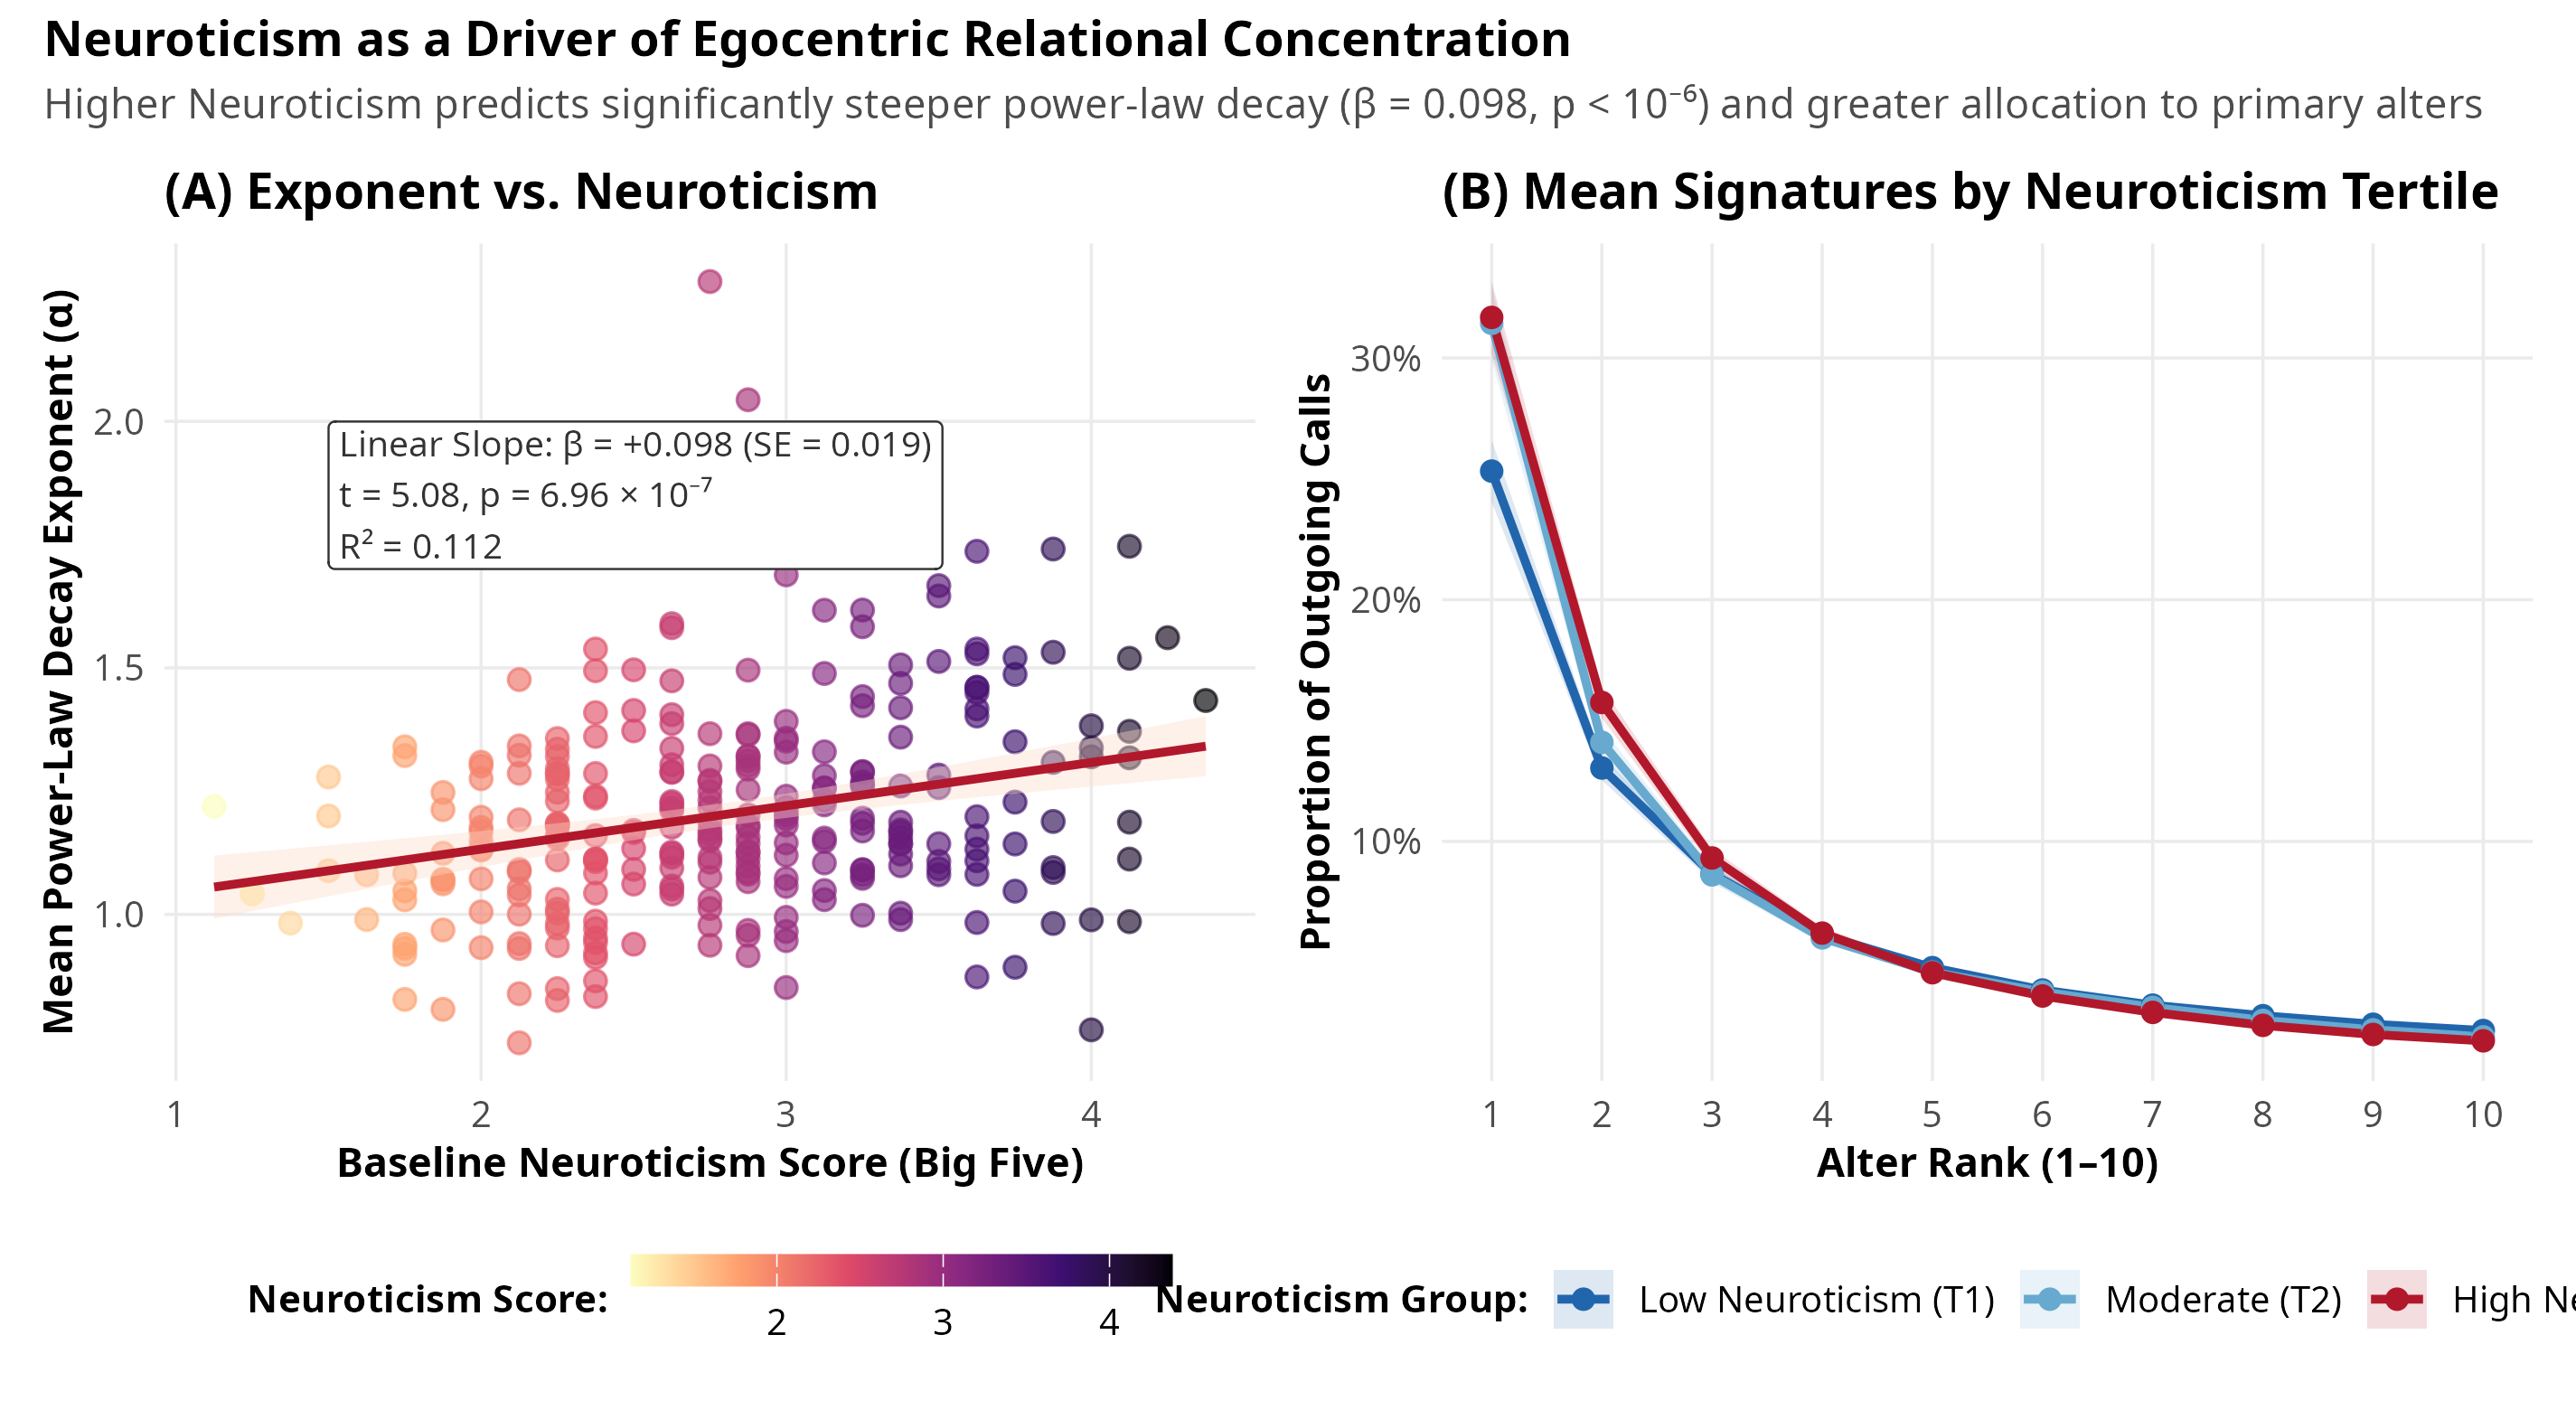
\includegraphics[width=0.92\textwidth]{Plots/fig07_personality_signature_effects.png}
\caption{\textbf{Negative Emotionality as a Driver of Egocentric Relational Concentration ($N = 290$ Egos).} \textbf{a}, Scatterplot and linear regression of mean power-law decay exponent ($\alpha_i$) on baseline Negative Emotionality ($\beta = 0.098, t = 5.08, p < 0.0001, R^2 = 0.112$), demonstrating that individuals higher in negative emotionality maintain systematically steeper decay profiles. \textbf{b}, Mean empirical social signatures across alter ranks 1 through 10 contrasting students in the highest tertile (T3, orange) versus lowest tertile (T1, blue) of Negative Emotionality, showing that high Negative Emotionality individuals direct 31.7\% of all communication to their single primary alter, compared to 25.3\% for low Negative Emotionality peers.}
\label{fig:personality}
\end{figure}

Contrasting students at the extremes of Negative Emotionality confirms this behavioral shift (Figure~\ref{fig:personality}b): students in the highest tertile (T3) direct an average of 31.7\% of outgoing communication to their single top alter (and 15.7\% to Rank 2), compared to 25.3\% at Rank 1 (and 13.0\% at Rank 2) for students in the lowest tertile (T1). In contrast, Extraversion displays no statistically significant linear main effect ($\beta = -0.017, t = -1.01, p = 0.314$), indicating that outgoing sociability does not linearly alter signature curvature.

To examine potential non-linear interactions, we trained a regression tree (Classification and Regression Tree; CART) predicting power-law decay exponents ($\alpha_i$) from baseline Big Five traits (Extended Data Fig.~\ref{fig:cart_tree}). The CART model confirms the primacy of Negative Emotionality (49\% relative variable importance), forming the root partition at a cutoff of 2.44. For low scorers ($< 2.44$, $n = 98$), attention remains egalitarian ($\bar{\alpha} = 1.121$). Among individuals with elevated Negative Emotionality ($\ge 2.44$, $n = 192$), the tree splits conditionally on Extraversion at 2.56: introverts ($< 2.56$, $n = 40$) exhibit extreme relational concentration ($\bar{\alpha} = 1.322$, rising to $1.392$ when combined with high Agreeableness), whereas moderate-to-high Extraversion ($\ge 2.56$, $n = 152$) acts as a psychological buffer against hyper-concentration ($\bar{\alpha} = 1.223$). This non-linear buffering dynamic clarifies why Extraversion showed no linear main effect, as it operates conditionally among individuals prone to emotional distress.

\section*{Discussion}

By pairing continuous passive smartphone logs with multi-wave ego-network surveys and psychological inventories in the NetHealth cohort, this study provides empirical grounding for social signature theory while advancing the paradigm into social network analysis and computational psychology. The findings resolve long-standing theoretical puzzles regarding how personal networks balance relational fluidity with structural stability across major life transitions.

Our results establish that social signatures represent an enduring individual-level regularity that holds across a nested hierarchy of observational timescales. Across all eight temporal window definitions, intraindividual self-divergence is systematically smaller than interindividual reference divergence ($p < 0.0001$), with stability persisting from coarse-grained annual scales ($\dself = 0.0633$) down to fine-grained three-week rolling windows ($\dself = 0.0495$). Furthermore, parametric evaluations clarify the mathematical morphology of communication allocation: power-law decay models ($R^2 = 0.935$) decisively outperform exponential models ($R^2 = 0.746$), with power-law scaling preferred by AIC in 97.0\% of semester specifications. Crucially, tracking cumulative observation intervals across 24 consecutive months shows that estimated decay parameters converge asymptotically within six to eight months of continuous digital observation, establishing a rigorous empirical burn-in guideline for subsequent personal network sensing studies.

More importantly, our findings resolve the content black box that has constrained passive digital sensing research. By linking 13,174 call-ranked dyads to longitudinal ego-network surveys across six signature Dunbar tiers, we show that communication ranks delineate sharp, qualitative boundaries in relational content, social support, and cognitive accessibility. The top-ranked alter constitutes a specialized kinship-dominated support hub (69.7\% family, primarily parents and partners), providing the structural backbone of instrumental advice (87.6\%), emotional support (85.4\%), and financial assistance (64.1\%). Ranks 2 and 3 represent the sympathy group, retaining high kinship density (62.2\%) and emotional comfort (77.1\%). Between Ranks 3 and 5, personal networks undergo a structural transition toward peer friendship dominance (rising from 56.9\% to 87.8\% in outer ranks). Notably, while emotional and advisory support decline monotonically across tiers, companionship remains elevated across all tiers (averaging over 69\% even beyond Rank 20), demonstrating that peripheral communication serves vital recreational and social integration functions rather than casual acquaintance.

Hierarchical mixed-effects models further reveal that signature position slots reflect deep evaluative and cognitive alignment. Relationship longevity ($t = 30.26, p < 0.0001$), cognitive recall accessibility ($t = 23.47, p < 0.0001$), interpersonal trust ($t = 6.95, p < 0.0001$), and subjective closeness ($t = 4.73, p < 0.0001$) each exert strong, independent positive effects on communication allocation. Over 93\% of primary alters are rated as especially close and average 14.2 years of relational duration, compared to 52.7\% and 4.9 years for outer ties; furthermore, 71.2\% of primary alters are recalled within the first five alters elicited during surveys. These findings provide direct empirical support for classical network formulations of tie strength:\cite{granovetter1973strength,marsden1984measuring-f62,burt2000decay-f08} communication rank is the behavioral enactment of accumulated biographical capital, top-of-mind cognitive accessibility, and emotional intimacy.

Our analyses also provide direct empirical verification of the slot-filling mechanism. Despite an average semester-to-semester alter turnover of 80.1\%, participants maintain stable allocation profiles. Even when an individual experiences complete turnover of their primary confidant (Rank 1), self-divergence increases only marginally from 0.0431 to 0.0785. This demonstrates that personal networks possess a homeostatic structural equilibrium: the specific alters occupying the network are fluid and interchangeable, but the relational geometry governing attention allocation is persistent and enduring.\cite{fiske2004four-0f8} Multilevel panel models confirm that while turnover and activity shifts predict minor mutations in self-divergence, ego network clustering has no effect, indicating that signature stability is rooted in individual-level behavioral habits rather than the closure of the surrounding peer network.

Finally, uncovering the psychological foundations of signature curvature bridges the gap between individual personality dispositions\cite{mccrae2008empirical} and network morphology. In parametric regressions, Negative Emotionality strongly predicts steeper, core-concentrated allocation profiles ($\beta = 0.098, p < 0.0001$), indicating that individuals prone to anxiety and emotional vulnerability adopt a defensive allocation strategy, focusing scarce emotional bandwidth on an exclusive confidant. Going beyond linear models, recursive partitioning reveals that this inward orientation is conditionally moderated by Extraversion: introversion exacerbates relational concentration ($\bar{\alpha} = 1.322$), whereas moderate-to-high Extraversion acts as a protective buffer ($\bar{\alpha} = 1.223$) that preserves broader social connectivity. In applied behavioral sensing, tracking personal social signatures offers a promising, non-invasive avenue for detecting disruptions in relational equilibrium and identifying early indicators of social withdrawal during critical life transitions.

Several methodological considerations suggest fruitful avenues for future research. First, our communication records are derived from outgoing voice calls on smartphones. While voice calls capture the high-bandwidth core of personal support networks, contemporary sociality is distributed across multiple mediated channels, including text messaging, instant messaging, and social media platforms. Multi-stream digital sensing will be valuable for establishing whether composite multichannel signatures exhibit greater structural stability or channel-specific functional specialization.\cite{heydari2018multichannel,li2022evidence} Second, our sample consists of undergraduate students at a residential university, where interaction is shaped by organizational structures (dorms, majors, classes) and relational mobility is unusually high. Extending this design to non-residential populations, working adults, and older cohorts will be necessary to establish the lifespan boundaries of social signature morphology. Third, while baseline personality predicts signature steepness, the causal interplay between psychological states and network structure may be bidirectional; future work should use continuous-time panel models to trace how shifts in signature concentration co-evolve with psychological well-being over time.

\section*{Methods}

\subsection*{The NetHealth cohort and data collection}
The NetHealth study recruited an incoming cohort of undergraduate students at the University of Notre Dame beginning in Fall 2015;\cite{liu2018network,purta2016experiences,faust2017exploring} comprehensive study design, instrumentation, and survey protocols are documented on the project website at \url{https://sites.nd.edu/nethealth/}. Participants consented to continuous digital sensing via smartphone call and messaging logs and wearable fitness trackers, alongside dense ego-network and psychometric surveys administered at regular intervals throughout their collegiate careers. 

Our analytical design links five primary data streams: (1) continuous communication logs capturing 498,237 outgoing voice call events collected from participant iOS devices spanning June 30, 2015, through July 2, 2017, across 491 unique egos; (2) comprehensive institutional academic calendar records documenting semester dates, examination periods, and breaks; (3) eight longitudinal waves of ego-network surveys recording 35,913 alter nominations; (4) complete alter-alter edge lists documenting 174,748 structural ties connecting peers within each respondent's personal egocentric network; and (5) longitudinal psychometric survey batteries measuring Big Five personality dimensions.

\subsection*{Temporal window definitions and eligibility criteria}
To evaluate social signature persistence across differing temporal resolutions, we constructed two complementary binning schemes. The first scheme relies on calendar-based windows spanning July 1, 2015 through June 30, 2017: two academic years (July 2015--June 2016 and July 2016--June 2017), four collegiate semesters (Fall 2015, Spring 2016, Fall 2016, Spring 2017), eight academic quarters, and 24 consecutive calendar months. The second scheme evaluates week-based windows spanning July 6, 2015 through July 2, 2017 across 104 Monday-to-Sunday weeks: 102 three-week rolling windows evaluated in one-week increments, 52 discrete two-week intervals, and 104 discrete one-week intervals.

To ensure that estimated signatures reflect meaningful communication structures, egos were required to meet two standard inclusion criteria: (a) a minimum of 2 active alters in every window ($k_{i,w} \ge 2$), and (b) an average call volume exceeding 10 calls per window. The broader sensing pool comprises $N = 491$ unique egos with voice calls. The collegiate semester timescale ($W = 4$) retains $N = 290$ participants, serving as our primary analytical cohort for all subsequent dyadic, structural, and psychological modeling. Monthly and rolling weekly windows retain $N = 147$ and $N = 88$ egos, respectively (Extended Data Table~\ref{tab:cohort_summary}). Direct benchmarking across calendar resolutions evaluated the common calendar cohort ($N = 147$ egos) present in all four schemes simultaneously.

\subsection*{Social signature computation and divergence metrics}
For ego $i$ in temporal window $w$, communication weights $w_{i,j,w}$ (measured as total outgoing voice calls) to alters $j = 1, \dots, k_{i,w}$ are sorted in descending order: $w_{i,(1),w} \ge w_{i,(2),w} \ge \dots \ge w_{i,(k),w}$. The social signature is defined as the normalized vector of interaction proportions:
\begin{equation}
p_{i,w}(r) = \frac{w_{i,(r),w}}{W_{i,w}}, \quad \text{where } W_{i,w} = \sum_{j=1}^{k_{i,w}} w_{i,j,w} \quad \text{and} \quad \sum_{r=1}^{k_{i,w}} p_{i,w}(r) = 1
\end{equation}
where $r \in \{1, 2, \dots, k_{i,w}\}$ represents the alter rank.

To quantify the difference between two probability vectors $P = \{p_r\}_{r=1}^{k_1}$ and $Q = \{q_r\}_{r=1}^{k_2}$ of potentially unequal lengths, we append zeros to the shorter distribution up to length $K = \max(k_1, k_2)$ on-the-fly and compute the Jensen-Shannon Divergence:\cite{lin1991divergence}
\begin{equation}
\JSD(P \parallel Q) = H(M) - \frac{1}{2}\left[H(P) + H(Q)\right]
\end{equation}
where $M = \frac{1}{2}(P + Q)$ is the mixture distribution, and $H(P) = -\sum_{r=1}^{K} p_r \log_2(p_r)$ denotes Shannon entropy in bits (with $0 \log_2 0 \equiv 0$). JSD is symmetric, non-negative, and strictly bounded between 0 and 1 bit.

Self-divergence ($\dself$) measures the mean pairwise JSD between consecutive temporal windows for the same ego:
\begin{equation}
\dself(i) = \frac{1}{W-1} \sum_{w=1}^{W-1} \JSD(P_{i,w} \parallel P_{i,w+1})
\end{equation}
Reference-divergence ($\dref$) quantifies the divergence between social signatures of distinct individuals observed within the same temporal window:
\begin{equation}
\dref(i) = \frac{1}{W} \sum_{w=1}^W \left[ \frac{1}{n_w - 1} \sum_{j \neq i} \JSD(P_{i,w} \parallel P_{j,w}) \right]
\end{equation}

\subsection*{Parametric model fitting and burn-in analysis}
We evaluated two competing functional specifications for each empirical signature: power-law decay ($p(r) = c \cdot r^{-\alpha}$) and exponential decay ($p(r) = c \cdot e^{-\beta r}$). Models were estimated via nonlinear least squares and log-linear regression across all ego-window observations. Model selection was assessed using Akaike's Information Criterion (AIC) and the coefficient of determination ($R^2$). To determine parameter burn-in convergence, we tracked the common cohort ($N = 147$) across cumulative observation windows from 2 to 24 months, computing the mean absolute error (MAE) of the estimated decay parameter $\alpha$ relative to the 24-month asymptotic value.

\subsection*{Ego-network survey linkage and social support dimensions}
Longitudinal ego-network surveys were administered across eight waves. In each wave, respondents completed name generators eliciting personal contacts, followed by name interpreters capturing relationship role categories (family kin vs.\ peer friends), subjective closeness (1 = not close, 2 = somewhat close, 3 = close, 4 = especially close), interpersonal trust (1--10 scale), relationship duration in years, and specific provisions of social support. Social support was evaluated across four distinct dimensions: emotional support (confiding personal problems), instrumental/advisory support (seeking advice or guidance), social companionship (spending leisure time together), and financial support (loaning money or material aid). Surveys were linked to phone call records by matching anonymized participant and alter identifiers within each collegiate semester window, yielding $N = 13,174$ call-ranked dyadic observations across 283 unique egos.

\subsection*{Dyadic linear mixed-effects models}
To model communication allocation while accounting for the hierarchical clustering of ties within participants ($N = 10,828$ complete dyads across $J = 280$ individuals), we estimated linear mixed-effects models with ego random intercepts using the \texttt{lme4} package\cite{bates2015fitting} in \textsf{R};\cite{Rmanual}
\begin{equation}
y_{ij} = \beta_0 + \mathbf{X}_{ij}\boldsymbol{\beta} + u_i + \epsilon_{ij}
\end{equation}
where $y_{ij}$ denotes the calling proportion $p_{ij}$ or ordinal signature rank $r_{ij}$ for alter $j$ of ego $i$, $\mathbf{X}_{ij}$ is a vector of dyadic attributes (closeness, trust, duration, recall salience), $u_i \sim \mathcal{N}(0, \tau_{00})$ is the ego random intercept, and $\epsilon_{ij} \sim \mathcal{N}(0, \sigma^2)$ is the residual error. Intraclass correlations were calculated as $\text{ICC} = \tau_{00} / (\tau_{00} + \sigma^2)$.

\subsection*{Multilevel longitudinal panel models}
To identify the structural determinants of signature mutation over time, we estimated multilevel linear mixed-effects panel models predicting Jensen-Shannon self-divergence ($\JSD_{it}$) across consecutive semesters ($N = 870$ transitions across 290 egos):
\begin{equation}
\JSD_{it} = \beta_0 + \beta_1 \Turnover_{it} + \beta_2 \Delta \mathrm{Activity}_{it} + \mathbf{X}_{it}\boldsymbol{\gamma} + u_i + \epsilon_{it}
\end{equation}
where $\Turnover_{it}$ is the dyadic Jaccard alter turnover, $\Delta \mathrm{Activity}_{it}$ is the absolute percentage change in total call volume ($|\Delta\mathrm{Calls}|/\mathrm{Calls}$), and $\mathbf{X}_{it}$ captures ego network clustering, network density, and baseline personality traits.

\subsection*{Psychometric assessments and recursive partitioning}
Personality dimensions were assessed at baseline using the Big Five Inventory (BFI-2), measuring Extraversion, Agreeableness, Conscientiousness, Negative Emotionality, and Openness on standardized 1--5 Likert scales. To examine non-linear psychological interactions predicting mean power-law decay exponents ($\alpha_i$), we trained a Classification and Regression Tree (CART)\cite{breiman1984classification} using the \texttt{rpart} package in \textsf{R}. The tree was grown with a minimum split size of 20 and pruned using 10-fold cross-validation to prevent overfitting.

\subsection*{Ethics, consent, and institutional review}
The NetHealth study was reviewed and approved by the Institutional Review Board (IRB) at the University of Notre Dame (Protocol \#15-05-2556). All participants provided written informed consent prior to data collection, including explicit authorization for continuous smartphone communication logging, wearable sensor tracking, and longitudinal survey administration. Data were fully anonymized with cryptographic hashing prior to analytical processing.

\section*{Data Availability}
The data analyzed in this study are derived from the NetHealth project. Information regarding the study data, instrumentation, and access protocols is available at the NetHealth project website hosted at the University of Notre Dame (\url{https://sites.nd.edu/nethealth/}).

\section*{Code Availability}
All custom \textsf{R} scripts used for data preprocessing, social signature computation, Jensen-Shannon divergence calculations, parametric model fitting, dyadic mixed-effects regressions, and recursive partitioning are deposited in a publicly accessible GitHub repository at \url{https://github.com/olizardo/social-signatures-nethealth} and will be permanently archived on Zenodo upon publication.

\section*{Acknowledgements}
This research was supported by the National Institutes of Health (NIH Grant R01HL117757). We thank the NetHealth research team at the University of Notre Dame, including Tijana Milenkovi{\'c}, Christian Poellabauer, Aaron Striegel, and Nitesh Chawla, for their leadership in study design and data infrastructure.

\section*{Author Contributions}
O.L. and D.H. conceptualized the study, designed the analytical framework, developed the methodology, performed statistical analyses, interpreted the results, and wrote the manuscript. Both authors reviewed and approved the final manuscript.

\section*{Competing Interests}
The authors declare no competing interests.

% --- References ---
\bibliographystyle{unsrtnat}
\bibliography{references}

\newpage

% --- Extended Data Section ---
\section*{Extended Data}

\renewcommand{\figurename}{Extended Data Fig.}
\renewcommand{\tablename}{Extended Data Table}
\setcounter{figure}{0}
\setcounter{table}{0}

\begin{table}[htbp]
\centering
\caption{\textbf{NetHealth Cohort Summary Across Temporal Window Definitions}}
\label{tab:cohort_summary}
\small
\resizebox{\textwidth}{!}{%
\begin{tabular}{lcccc}
\toprule
\textbf{Window Scheme} & \textbf{Window Span} & \textbf{Windows ($W$)} & \textbf{Eligibility Criteria} & \textbf{Eligible Egos ($N$)} \\
\midrule
Academic Years & Jul 2015 -- Jun 2017 & 2 & $\ge 2$ alters, $>10$ calls & 388 \\
Semesters & Jul 2015 -- Jun 2017 & 4 & $\ge 2$ alters, $>10$ calls & 290 \\
Quarters & Jul 2015 -- Jun 2017 & 8 & $\ge 2$ alters, $>10$ calls & 227 \\
Months & Jul 2015 -- Jun 2017 & 24 & $\ge 2$ alters, $>10$ calls & 147 \\
Common Calendar Cohort & Jul 2015 -- Jun 2017 & -- & All 4 calendar schemes & 147 \\
3-Week Rolling & Jul 2015 -- Jul 2017 & 102 & $\ge 2$ alters, $>10$ calls & 88 \\
2-Week Discrete & Jul 2015 -- Jul 2017 & 52 & $\ge 2$ alters, $>10$ calls & 65 \\
1-Week Discrete & Jul 2015 -- Jul 2017 & 104 & $\ge 2$ alters, $>10$ calls & 14 \\
\bottomrule
\end{tabular}%
}
\end{table}

\begin{table}[htbp]
\centering
\caption{\textbf{Statistical Tests of Social Signature Persistence Across Window Schemes}}
\label{tab:stability_tests}
\small
\resizebox{\textwidth}{!}{%
\begin{tabular}{lcccccc}
\toprule
\textbf{Scheme} & \textbf{Egos ($N$)} & \textbf{Mean $\dself$ (SD)} & \textbf{Mean $\dref$ (SD)} & \textbf{Difference} & \textbf{Wilcoxon $V$} & \textbf{$p$-value} \\
\midrule
Academic Years & 388 & 0.0633 (0.0642) & 0.1129 (0.0322) & $-0.0496$ & 6,690.0 & $< 0.0001$ \\
Semesters & 290 & 0.0614 (0.0423) & 0.1184 (0.0304) & $-0.0570$ & 1,136.0 & $< 0.0001$ \\
Quarters & 227 & 0.0626 (0.0311) & 0.1293 (0.0299) & $-0.0667$ & 50.0 & $< 0.0001$ \\
Months & 147 & 0.0877 (0.0305) & 0.1494 (0.0248) & $-0.0617$ & 14.0 & $< 0.0001$ \\
Common Cohort (Sem) & 147 & 0.0458 (0.0244) & 0.1057 (0.0250) & $-0.0599$ & 30.0 & $< 0.0001$ \\
Common Cohort (Mo) & 147 & 0.0877 (0.0305) & 0.1494 (0.0248) & $-0.0617$ & 14.0 & $< 0.0001$ \\
3-Week Rolling & 88 & 0.0495 (0.0147) & 0.1411 (0.0205) & $-0.0916$ & 0.0 & $< 0.0001$ \\
2-Week Discrete & 65 & 0.0992 (0.0216) & 0.1439 (0.0167) & $-0.0447$ & 0.0 & $< 0.0001$ \\
\bottomrule
\end{tabular}%
}
\end{table}

\begin{table}[htbp]
\centering
\caption{\textbf{Parametric Model Evaluation Across Window Resolutions}}
\label{tab:parametric_models}
\small
\begin{tabular}{lcccccc}
\toprule
\textbf{Scheme} & \textbf{Models ($N$)} & \textbf{Power-Law $\alpha$ (SD)} & \textbf{Power-Law $R^2$} & \textbf{Exp $\beta$} & \textbf{Exp $R^2$} & \textbf{\% PL Preferred} \\
\midrule
Semesters & 1,158 & 1.20 (0.26) & 0.935 & 0.10 & 0.746 & 97.0\% \\
Months & 3,496 & 1.06 (0.37) & 0.883 & 0.23 & 0.771 & 83.8\% \\
\bottomrule
\multicolumn{7}{l}{\footnotesize Preference evaluated via Akaike's Information Criterion (AIC).}
\end{tabular}
\end{table}

\begin{figure}[htbp]
\centering
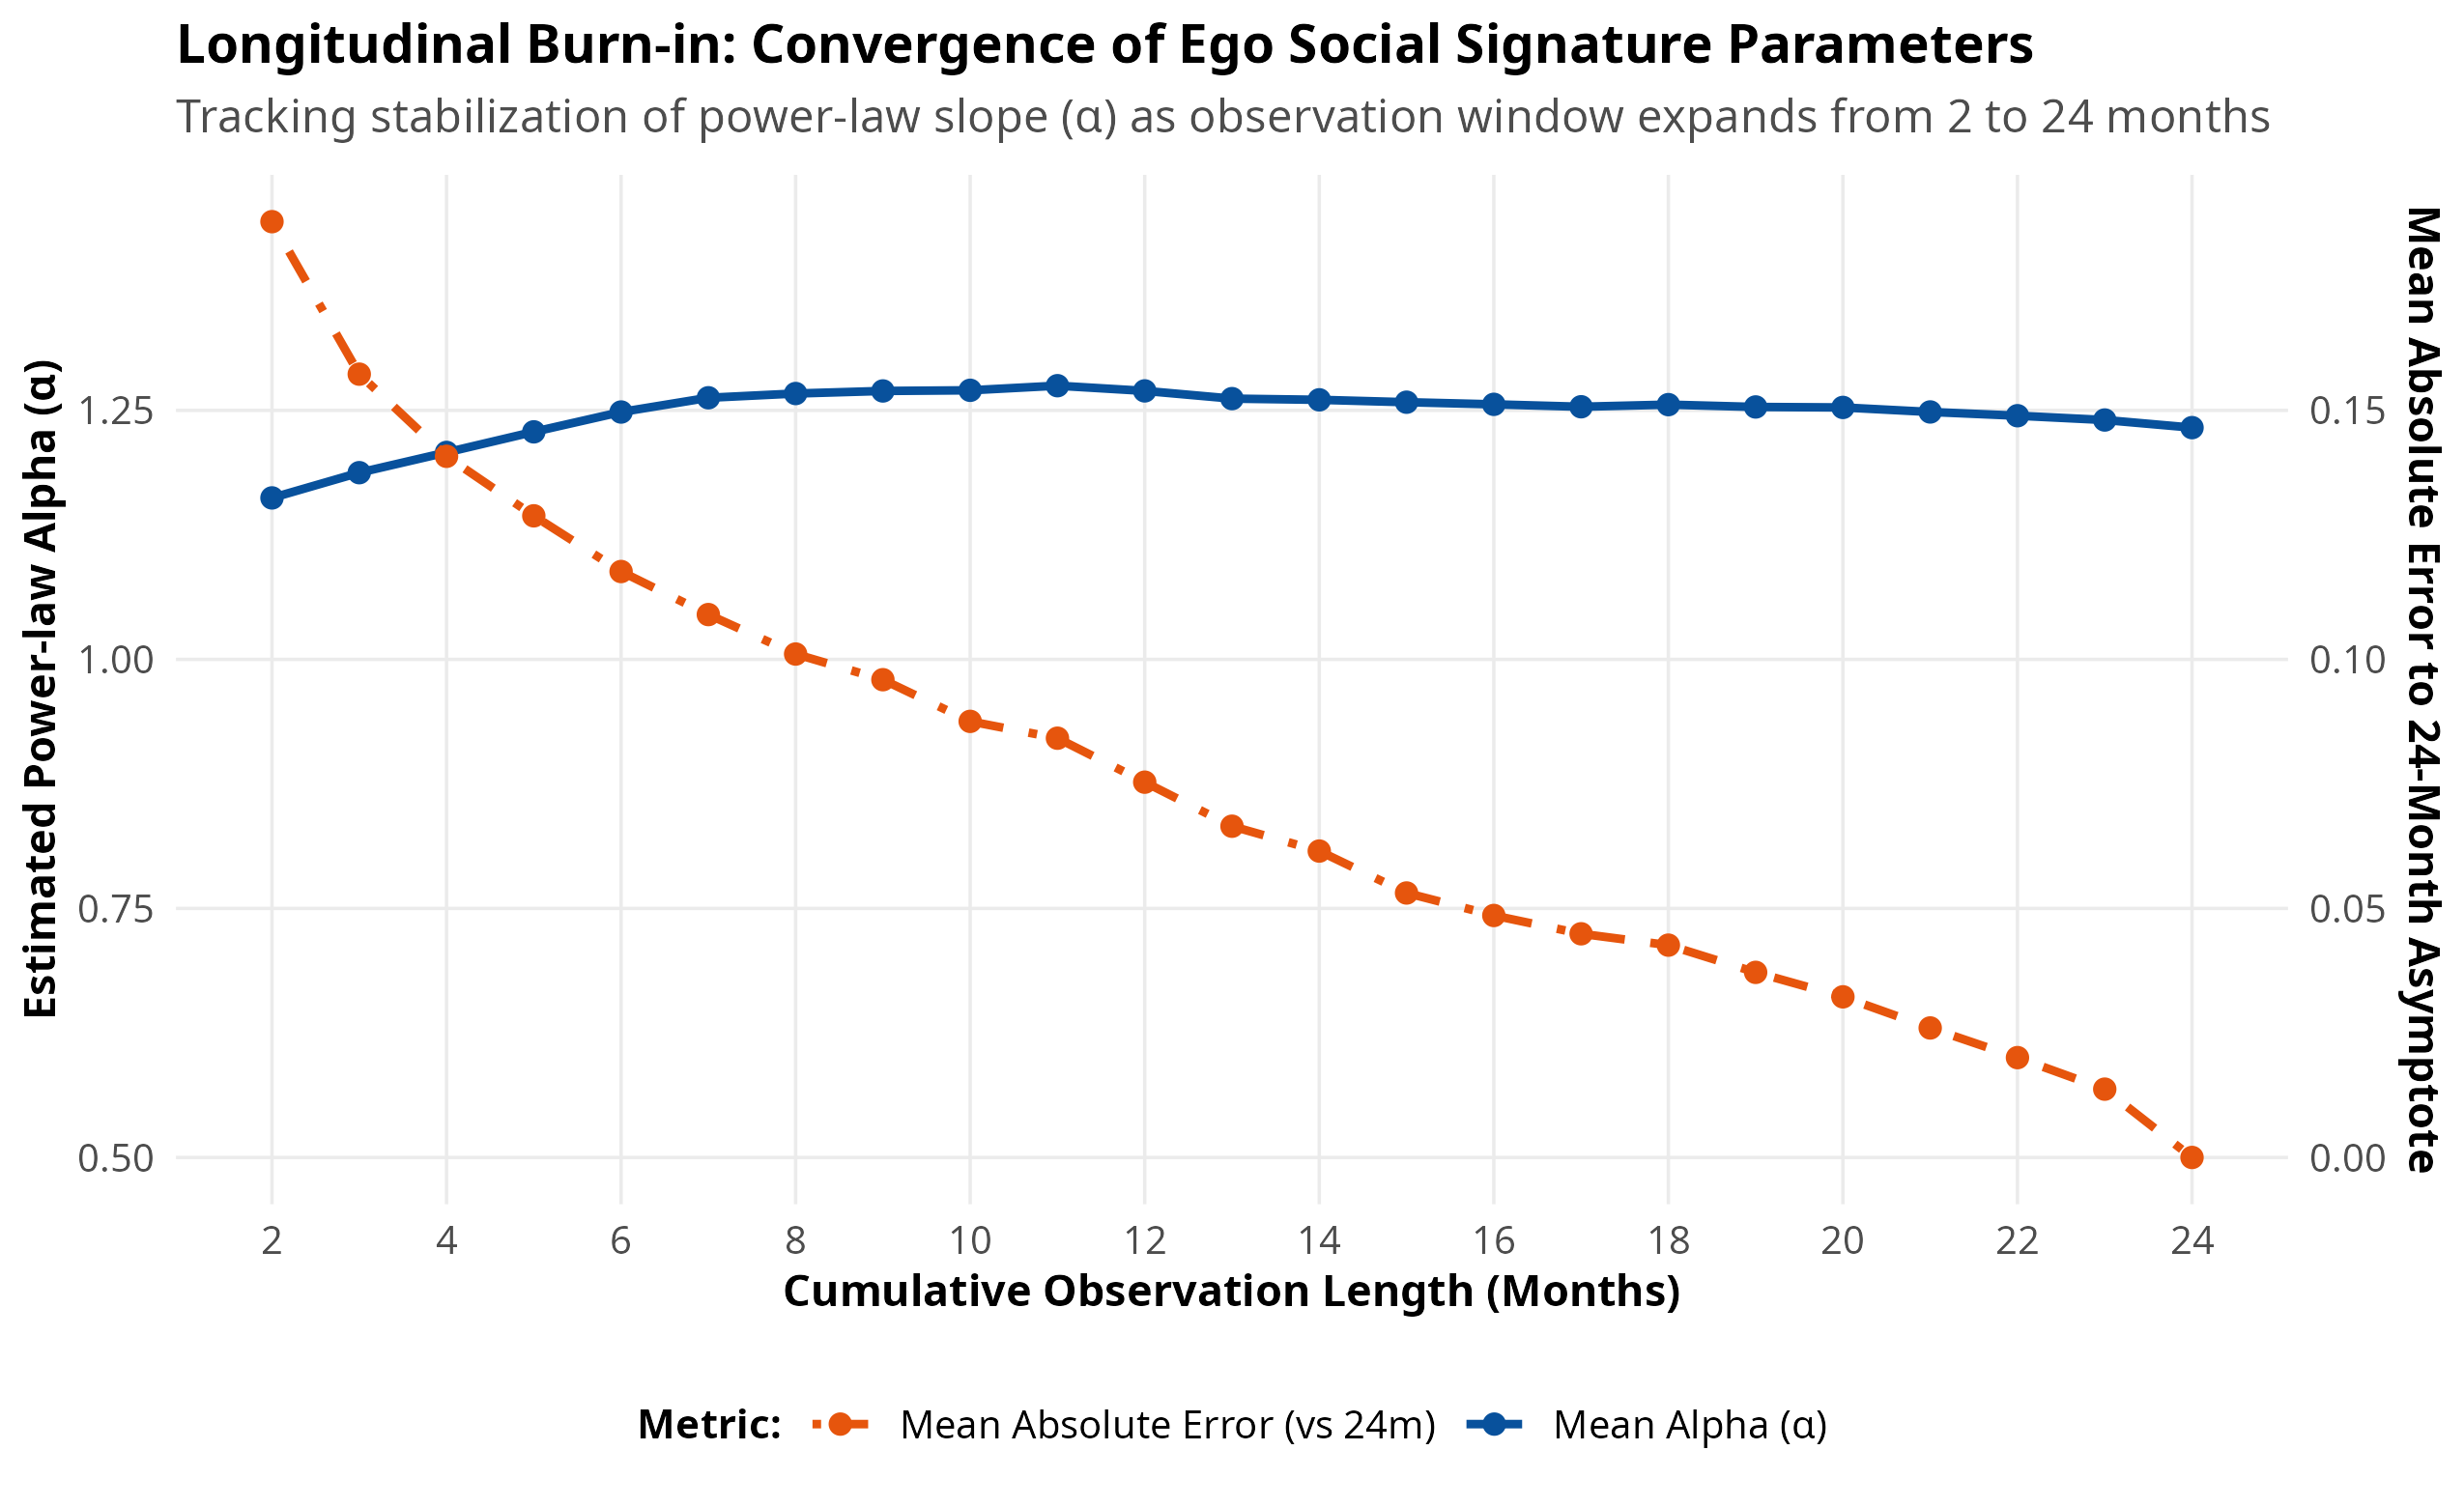
\includegraphics[width=0.88\textwidth]{Plots/fig04_parameter_burnin.png}
\caption{\textbf{Parameter Burn-In Convergence Over 24 Months.} Left axis shows mean estimated power-law decay exponent ($\alpha$); right axis shows mean absolute error relative to the 24-month asymptotic parameter value across cumulative observation intervals from 2 to 24 months ($N = 147$ common cohort). Estimates stabilize within six to eight months.}
\label{fig:burnin}
\end{figure}

\begin{figure}[htbp]
\centering
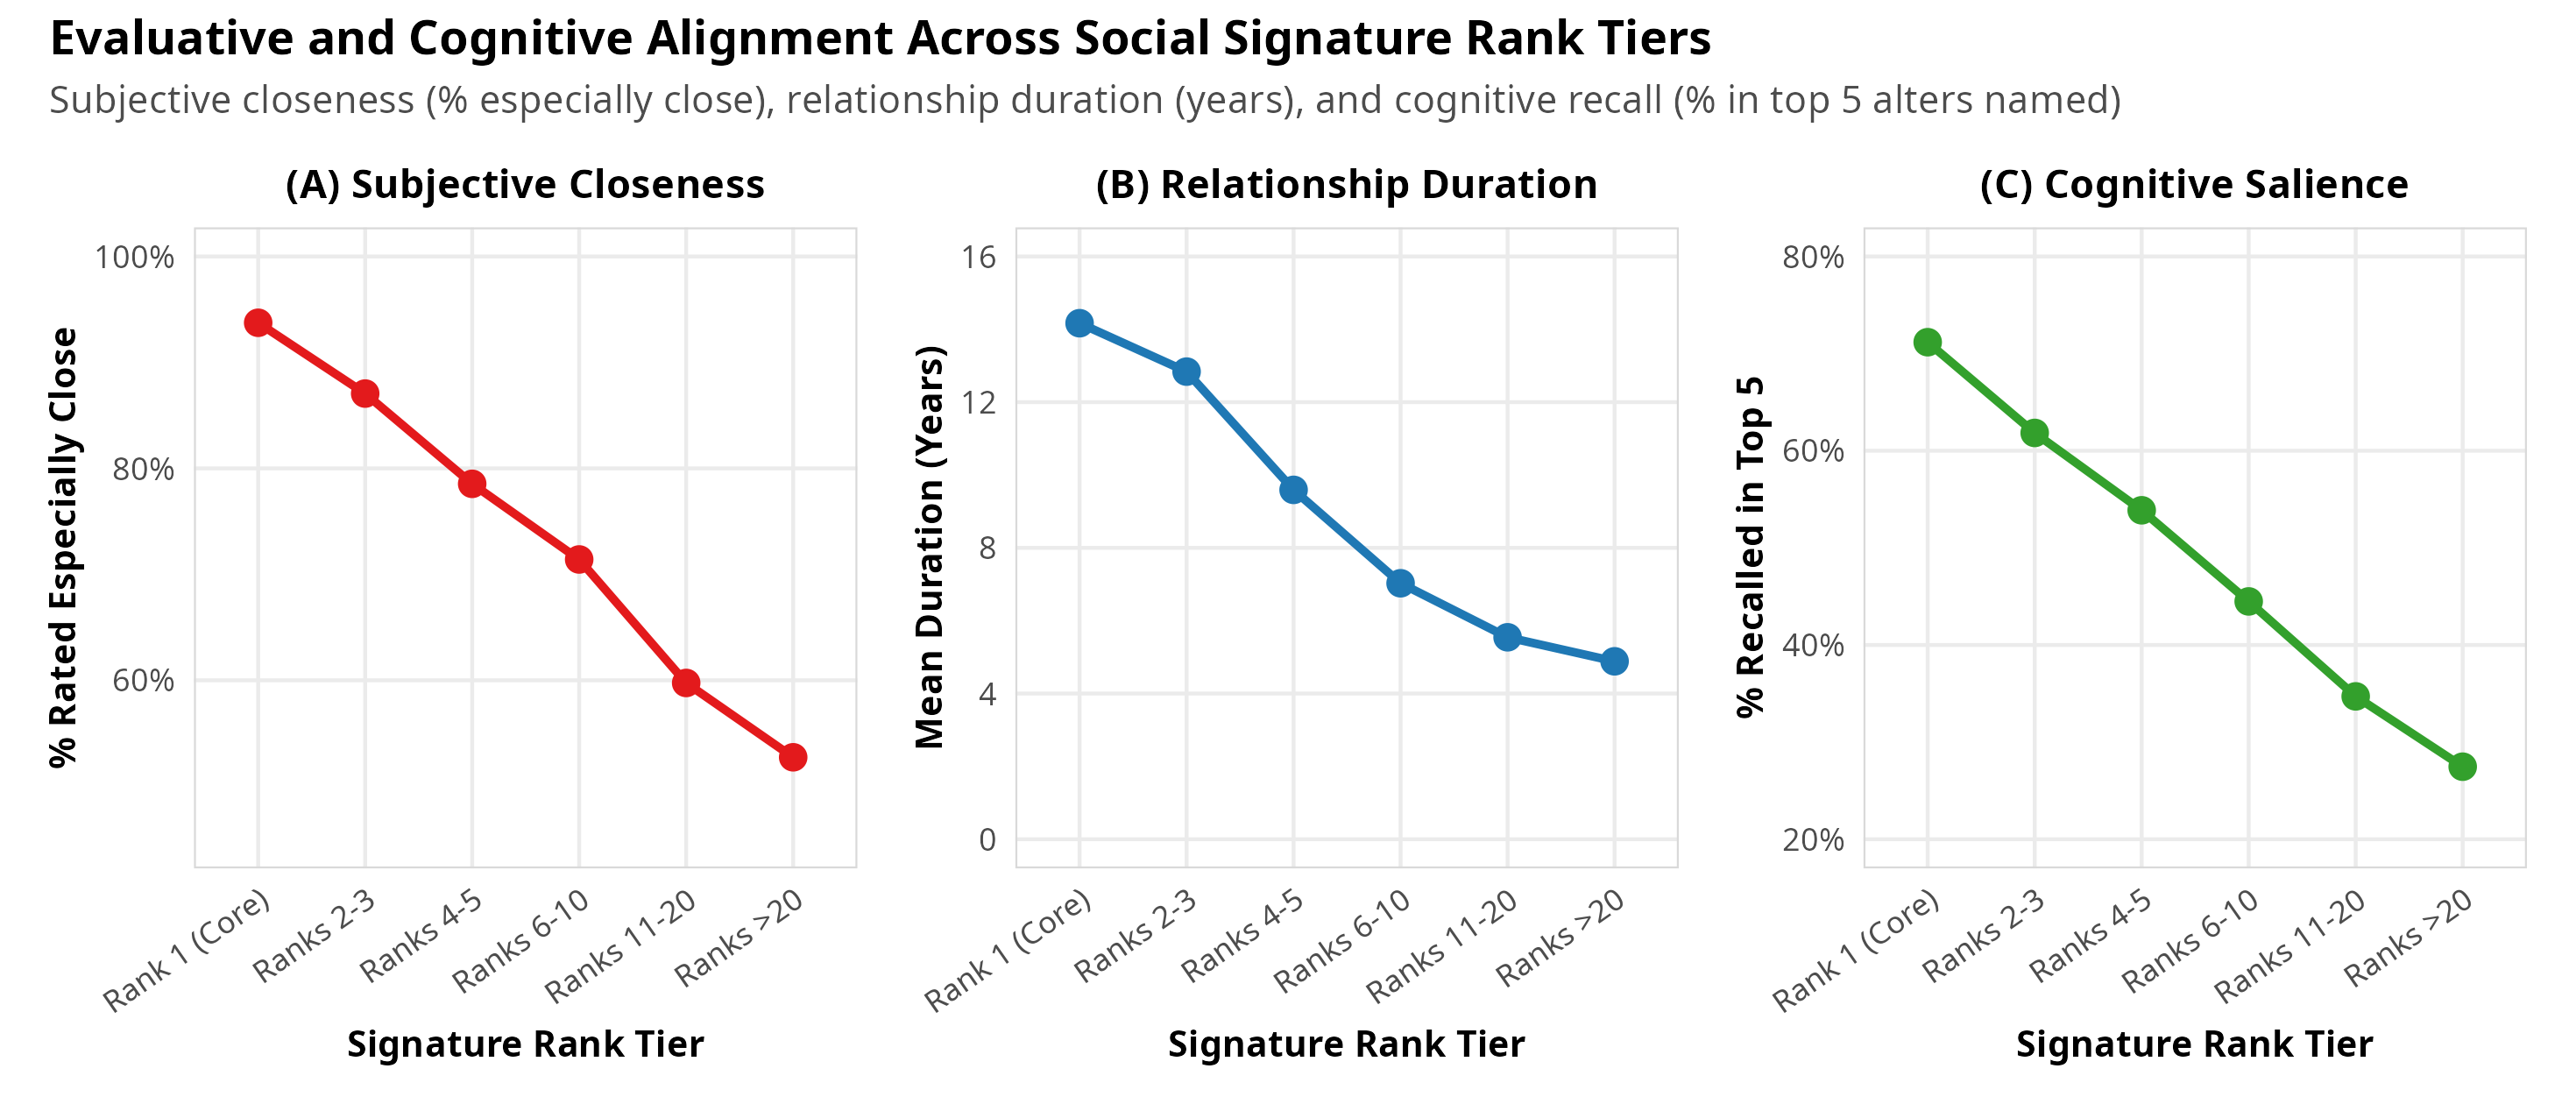
\includegraphics[width=0.95\textwidth]{Plots/fig05b_closeness_duration_salience.png}
\caption{\textbf{Evaluative and Cognitive Alignment Across Social Signature Rank Tiers ($N = 13,174$ Dyads).} \textbf{a}, Subjective Closeness: percentage of alters rated as ``especially close'' on a 1--4 scale. \textbf{b}, Relationship Duration: mean relationship longevity in years. \textbf{c}, Cognitive Salience: percentage of alters recalled within the top 5 positions during survey elicitation.}
\label{fig:tie_evaluative}
\end{figure}

\begin{table}[htbp]
\centering
\caption{\textbf{Multilevel Linear Mixed-Effects Models Predicting Signature Self-Divergence ($\JSD$)}}
\label{tab:multilevel_models}
\small
\resizebox{\textwidth}{!}{%
\begin{tabular}{lccc}
\toprule
\textbf{Predictor Term} & \textbf{Model 1 (Turnover)} & \textbf{Model 2 (Topology)} & \textbf{Model 3 (Integrated)} \\
\midrule
Intercept & $-0.237^{***}\ (0.0195)$ & $-0.200^{***}\ (0.0224)$ & $-0.171^{***}\ (0.0320)$ \\
Alter Turnover ($1 - \Jaccard$) & $0.373^{***}\ (0.0242)$ & $0.336^{***}\ (0.0240)$ & $0.351^{***}\ (0.0287)$ \\
\% Activity Change ($|\Delta\mathrm{Calls}|/\mathrm{Calls}$) & -- & $0.0014^{***}\ (0.0002)$ & $0.0014^{***}\ (0.0002)$ \\
Ego Network Clustering Coefficient & -- & $-0.0145\ (0.0157)$ & $-0.0066\ (0.0153)$ \\
Ego Network Density & -- & $0.0029\ (0.0154)$ & -- \\
Baseline Extraversion & -- & -- & $-0.0048\ (0.0030)$ \\
Baseline Negative Emotionality & -- & -- & $-0.0088^{**}\ (0.0033)$ \\
\midrule
Transitions ($N$) & 870 & 870 & 870 \\
Ego Clusters ($J$) & 290 & 290 & 290 \\
\bottomrule
\multicolumn{4}{l}{\footnotesize Standard errors in parentheses. $^{***}p < 0.001$, $^{**}p < 0.01$, $^*p < 0.05$, $^\dagger p < 0.10$.}
\end{tabular}%
}
\end{table}

\begin{table}[htbp]
\centering
\caption{\textbf{Personality Determinants of Social Signature Power-Law Alpha ($\alpha_i$)}}
\label{tab:personality_models}
\small
\begin{tabular}{lcccc}
\toprule
\textbf{Term} & \textbf{Estimate} & \textbf{Std.\ Error} & \textbf{$t$ value} & \textbf{$p$-value} \\
\midrule
(Intercept) & $0.680^{***}$ & 0.162 & 4.21 & $< 0.001$ \\
Extraversion & $-0.017$ & 0.017 & $-1.01$ & 0.314 \\
Negative Emotionality & $0.098^{***}$ & 0.019 & 5.08 & $< 0.001$ \\
Agreeableness & $0.063^{*}$ & 0.025 & 2.49 & 0.014 \\
Conscientiousness & 0.021 & 0.023 & 0.89 & 0.374 \\
Openness & 0.014 & 0.027 & 0.53 & 0.598 \\
Personal Network Degree & $-0.004^\dagger$ & 0.002 & $-1.76$ & 0.080 \\
\midrule
\multicolumn{5}{l}{\footnotesize $N = 290$ egos, $R^2 = 0.124, F(6, 283) = 6.69, p < 0.0001$.}
\end{tabular}
\end{table}

\begin{figure}[htbp]
\centering
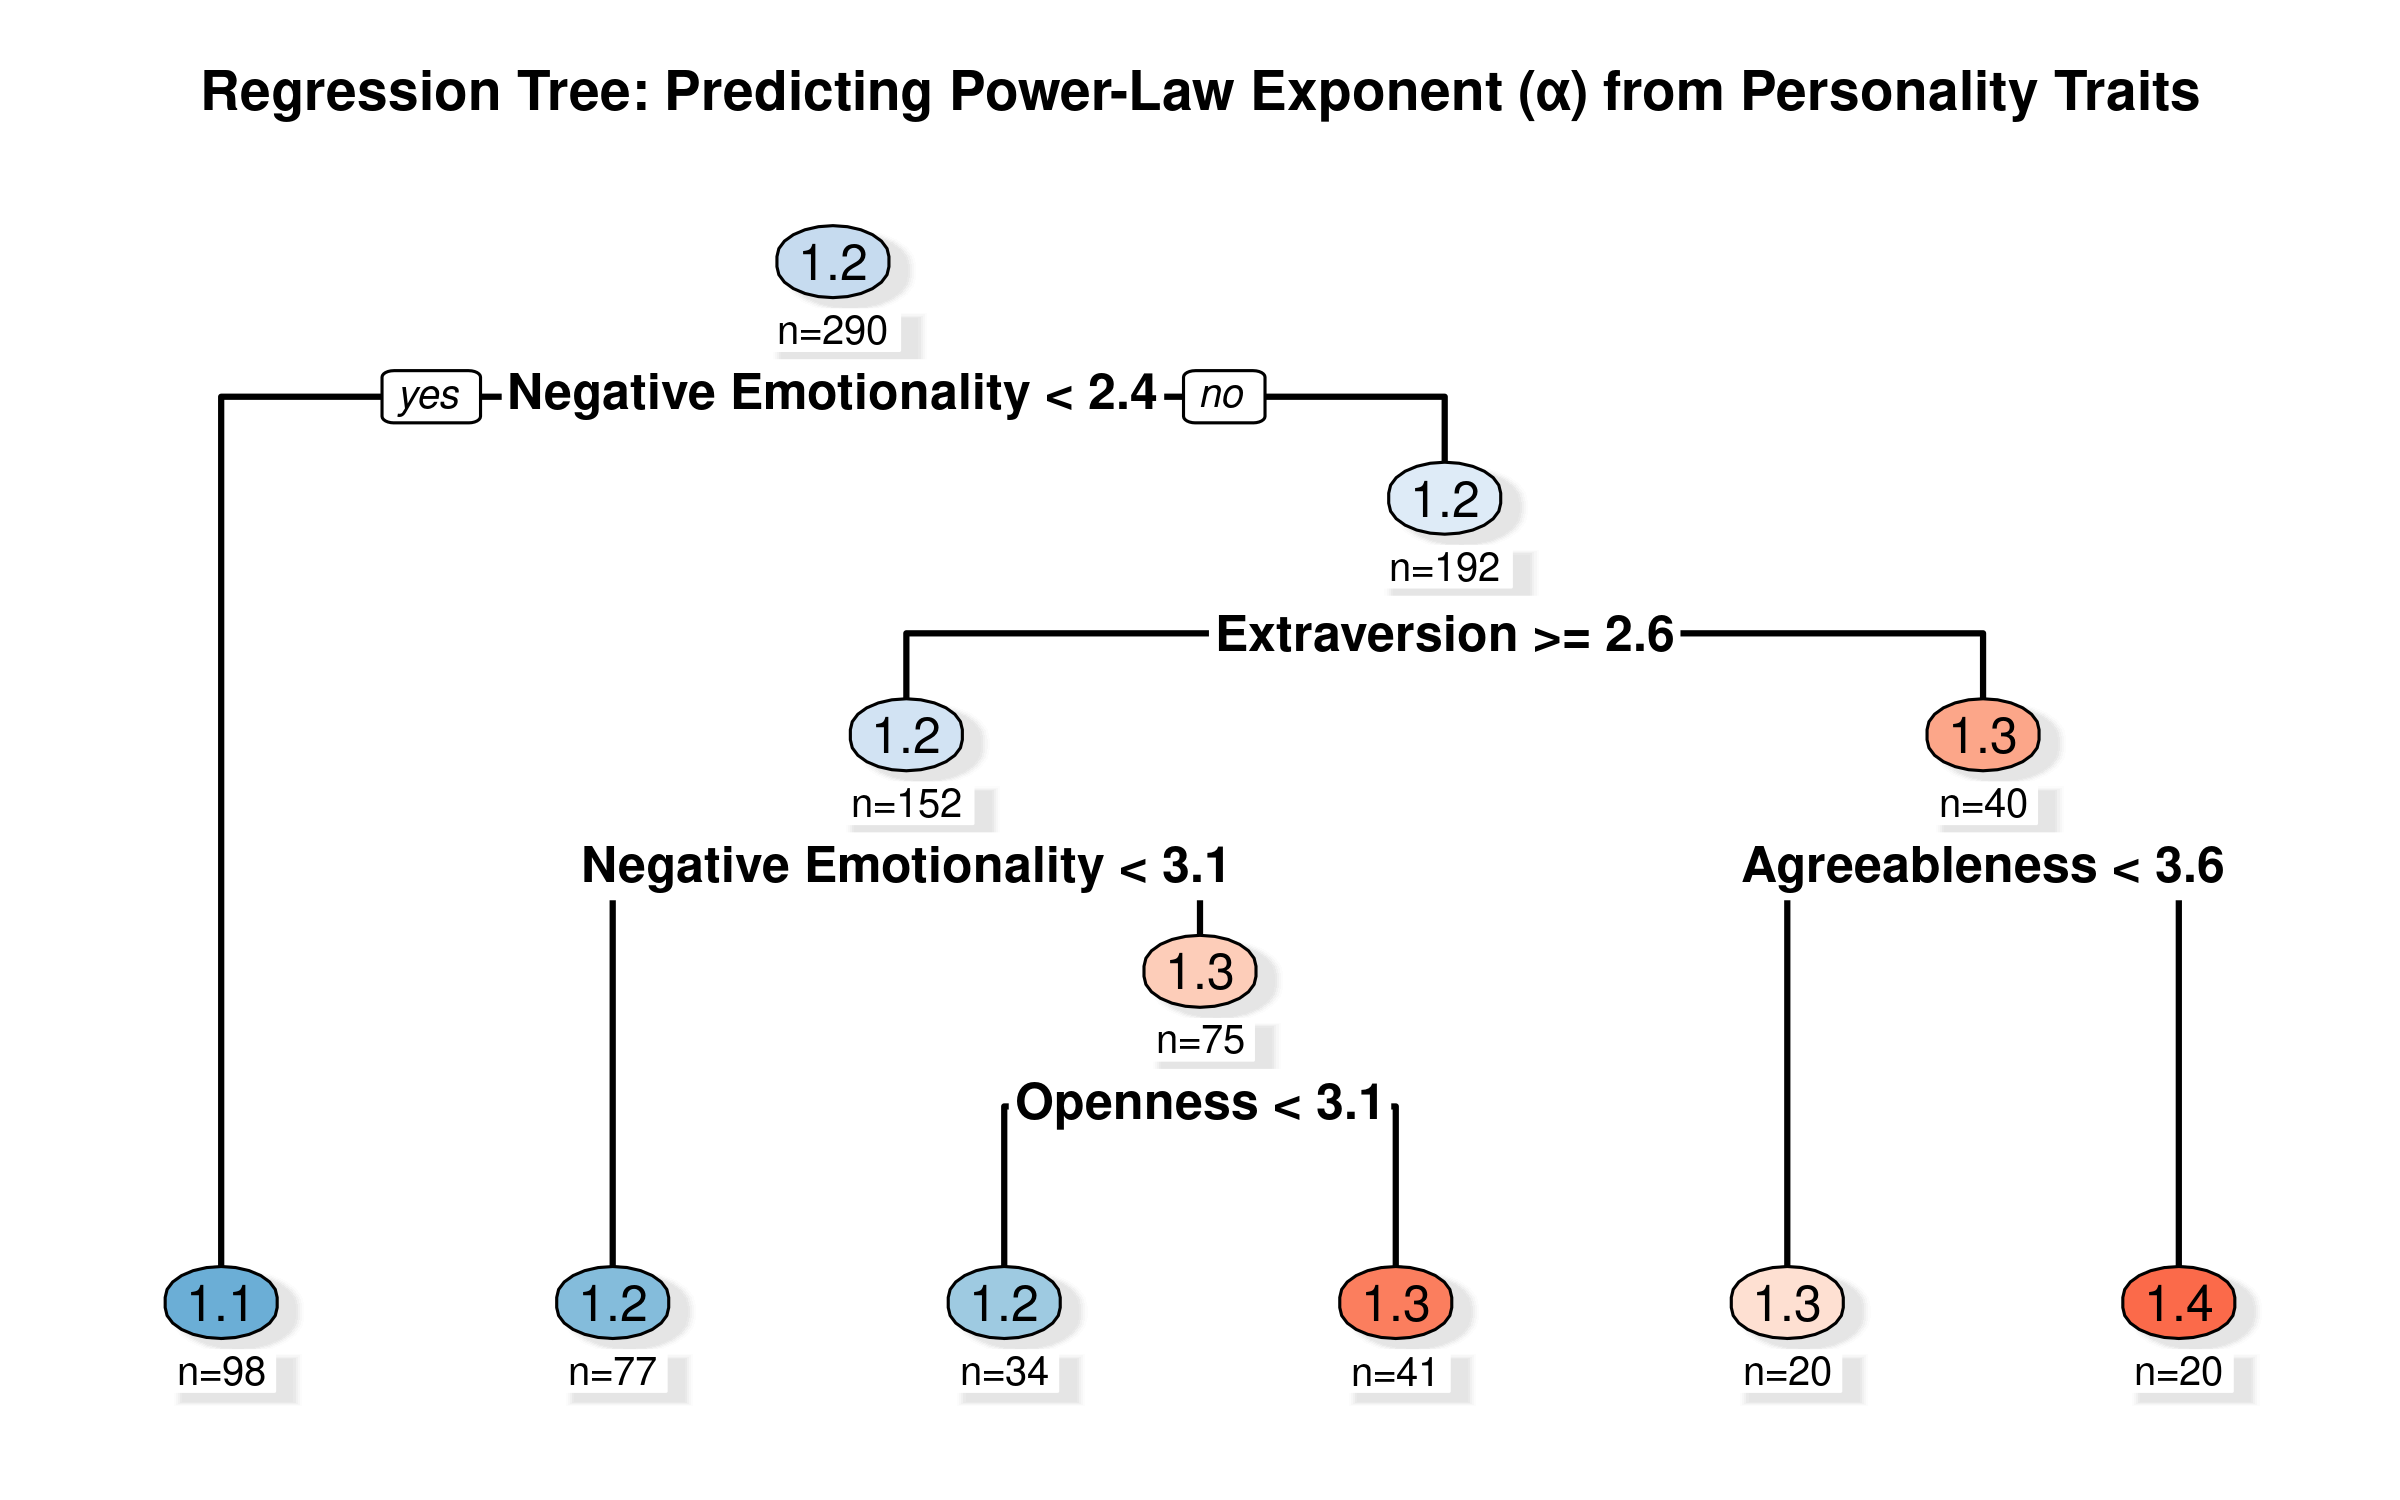
\includegraphics[width=0.92\textwidth]{Plots/fig08_cart_decision_tree.png}
\caption{\textbf{Classification and Regression Tree (CART) Predicting Social Signature Power-Law Alpha ($\alpha_i$) from Big Five Personality Traits ($N = 290$).} Node boxes display predicted mean $\alpha_i$ (top) and sample size (bottom), colored along a blue-to-red gradient from flat/egalitarian to steep/concentrated allocation profiles. Root split bifurcates on Negative Emotionality at 2.44, with conditional moderating split on Extraversion at 2.56.}
\label{fig:cart_tree}
\end{figure}

\end{document}
